%
%
%
\documentclass[3p]{elsarticle}
\linespread{1.5}

\usepackage{lineno,hyperref}

\journal{Journal of Statistical Planning and Inference}


\usepackage{graphicx}
%
\usepackage[misc]{ifsym}   % \Letter symbol
\usepackage{bm}
\usepackage{amsmath}
\usepackage{amssymb}
\usepackage{amsthm}
\usepackage{graphicx}
\usepackage{booktabs}
\usepackage[linesnumbered,ruled]{algorithm2e}
\usepackage{natbib}
\usepackage{appendix}
\usepackage{color}


\DeclareMathOperator{\mytr}{tr}
\DeclareMathOperator{\mydiag}{diag}
\DeclareMathOperator{\myrank}{Rank}
\DeclareMathOperator{\myE}{E}
\DeclareMathOperator{\myVar}{Var}

\newcommand{\BP}{\mathbf{P}}
\newcommand{\Bv}{\mathbf{v}}

\theoremstyle{plain}
\newtheorem{theorem}{\quad\quad Theorem}
\newtheorem{proposition}{\quad\quad Proposition}
\newtheorem{corollary}{\quad\quad Corollary}
\newtheorem{lemma}{Lemma}
\newtheorem{example}{Example}
\newtheorem{assumption}{\quad\quad Assumption}
\newtheorem{condition}{Condition}

\theoremstyle{definition}
\newtheorem{remark}{\quad\quad Remark}
\theoremstyle{remark}

\begin{document}




\begin{frontmatter}
\title{A feasible high dimensional randomization test for the mean vector}

\author[mymainaddress]{Rui Wang}
\author[mymainaddress,mysecondaryaddress]{Xingzhong Xu\corref{mycorrespondingauthor}}
\cortext[mycorrespondingauthor]{Corresponding author}
\ead{xuxz@bit.edu.cn}
\address[mymainaddress]{School of Mathematics and Statistics, Beijing Institute of Technology, Beijing 100081,China}
\address[mysecondaryaddress]{Beijing Key Laboratory on MCAACI, Beijing Institute of Technology, Beijing 100081,China}

\begin{abstract}
    The strength of randomization tests is that they are exact tests under certain symmetry assumption for distributions.
    In this paper, we propose a randomization test for the mean vector in high dimensional setting. 
    We give an implementation of the proposed randomization test procedure, which has low computational complexity.
    %In classical statistics, randomization tests are computationally intensive.    
    %Surprisingly, it is not the case in high dimensional setting. 
    %The theoretical property of the randomization test is another important issue.
    So far, the asymptotic behaviors of randomization tests have only been studied in fixed dimension case.
    We investigate the asymptotic behavior of the proposed randomization test in high dimensional setting.
    It turns out that even if the symmetry assumption is violated, the proposed randomization test still has correct level asymptotically.
    The asymptotic power function is also given.
    A simulation study is carried out to verify our theoretical results.
    

\end{abstract}

\begin{keyword}
   Asymptotic power function \sep High dimension \sep Randomization test\sep Symmetry assumption
\end{keyword}
\end{frontmatter}

\section{Introduction}

Suppose $X_{1},\ldots,X_{n}$ are $p$-variate independent and identically distributed (iid) random vectors with mean vector $\mu$ and covariance matrix $\Sigma$. In this paper, we consider the problem of testing the hypotheses
\begin{equation}\label{ourHy}
    H_0:\mu=0_p\quad \textrm{versus} \quad H_1:\mu\neq 0_p.
\end{equation}


%Tests for hypotheses~\eqref{ourHy} has been extensively studied by many researchers.
A classical test statistic for hypotheses~\eqref{ourHy} is Hotelling's $T^2$, defined as
    $
    n\bar{X}^T S^{-1}\bar{X}
    $,
where $\bar{X}=n^{-1}\sum_{i=1}^n X_i$ and $S=(n-1)^{-1}\sum_{i=1}^n (X_i-\bar{X}) (X_i-\bar{X})^T$ are the sample mean vector and sample covariance matrix, respectively.
Under normal distribution, Hotelling's $T^2$ is the likelihood ratio test and enjoys desirable properties in fixed $p$ setting. See, for example,~\citet{andersonMultivariate}.
However, Hotelling's test can not be defined when $p>n-1$ due to the singularity of $S$.
In a seminal paper,~\citet{Bai1996Efiect} considered two sample testing problem and proposed a statistic by removing $S^{-1}$ from Hotelling's $T^2$ statistic.
They studied the asymptotic properties of their test statistic when $p/n$ tends to a positive constant.
Many subsequent papers generalized the idea of~\citet{Bai1996Efiect} to more general models~\citep{Srivastava2008A,Chen2010A,Wang2015A}.
%\cite{Srivastava2007Multivariate} proposed a test based on $\bar{X} S^{+}\bar{X}$, where $S^{+}$ is the Moore-Penrose inverse of $S$.
%For example,~\cite{Srivastava2008A} proposed a test based on
%$
%\bar{X}^T {[\mathrm{diag}(S)]}^{-1} \bar{X}
%$,
%where $\mathrm{diag}(S)$ is the matrix with diagonal elements equal to that of $S$ and off-diagonal elements equal to $0$.
%\cite{Chen2010A} proposed a test based on $U$-statistic
%$\sum_{i\neq j}X_i^T X_j$.
%~\cite{Wang2015A} proposed a test based on  $\sum_{i\neq j}\|X_i\|^{-1}\|X_j\|^{-1}X_i^T X_j$.
%~\cite{Zhao2016A} proposed a test based on $\bar{X}^T (I_p-\BP_S)\bar{X}$, where $\BP_S$ is the orthogonal projection matrix on the column space of $S$.
%All these high dimensional statistics can be written as generalized quadratic forms of data, see~\cite{Jong1987A}. And the asymptotic properties of these statistics are mostly derived by martingale central limit theorem (MCLT).
The critical values of existing high dimensional tests are mostly determined by asymptotic distribution. 
We call it asymptotic method.
 In many real world problems, e.g., gene testing~\citep{efron2007on}, sample size $n$ may be very small.
In this case, the Type I error rate of the asymptotic method may be far away from nominal level. 

The randomization test method is a tool to determine the critical value for a given test statistic.
The idea of randomization tests dates back to~\citet{Fisher}.
See~\citet{Romano1990On} for a general construction of randomization test.
Its strength is in that the resulting test procedure has exact level under mild condition.
There are many papers concerning the theoretical properties of randomization tests for fixed $p$ case.
See, for example,~\citet{Romano1990On},~\citet{Zhu2000N} and~\citet{Chung2016Multivariate}.
In high dimensional setting, randomization tests are widely used in applied statistics~\citep{Subramanian2005,efron2007on,Ko2016}.
However, little is known about the theoretical properties of the randomization test in high dimensional setting.

In this paper, we consider the following randomization method.
Suppose $T(X_1,\ldots,X_n)$ is certain test statistic for hypotheses~\eqref{ourHy}.
Let $\epsilon_1,\ldots,\epsilon_n$ be iid Rademacher variables ($\Pr(\epsilon_i=1)=\Pr(\epsilon_i=-1)=1/2$) which are independent of data.
%Denote by
    %$
    %\mathcal{L}\big(T(\epsilon_1 X_1,\ldots,\epsilon_i X_i,\ldots,\epsilon_n X_n)|X_1,\ldots,X_n\big)
    %$
 %the distribution of $T(\epsilon_1 X_1,\ldots,\epsilon_i X_i,\ldots,\epsilon_n X_n)$ conditioning on $X_1,\ldots,X_n$.
 The randomization test rejects the null hypothesis when $T(X_1,\ldots, X_n)$ is greater than the $1-\alpha$ quantile of the conditional distribution of $T(\epsilon_1 X_1,\ldots,\epsilon_i X_i,\ldots,\epsilon_n X_n)$ with respect to $X_1,\ldots,X_n$,
 and accepts the null hypothesis otherwise, where $\alpha$ is the significant level and the $1-\alpha$ quantile of a distribution function $F(\cdot)$ is defined as $\inf\{y: F(y)\geq 1-\alpha\}$.
In fixed $p$ setting, it's well known that randomization tests consume much more computing time than the asymptotic method, which  historically  hampered the use of randomization tests. 
The goal of this paper is to show that in high dimensional setting, randomization tests can be computationally feasible and have desirable statistic properties.
Inspired by the work of~\citet{Bai1996Efiect} and~\citet{Chen2010A}, we propose a randomization test for hypotheses~\eqref{ourHy}.
We give a fast implementation of the proposed randomization test, the computational complexity of which is low.
When $p$ is large, our method even consumes less computing time  than the asymptotic method.
We also investigate the asymptotic behavior of the test procedure.
Our results show that even if the null distribution of $X_1$ is not symmetric, the randomization test is still asymptotically exact under mild assumptions. 
Hence the test procedure is robust.
The local asymptotic power function is also given.
To the best of our knowledge, this is the first work which gives the asymptotic behavior of randomization tests in high dimensional setting.
A simulation study is carried out to examine the numerical performance of the proposed randomization test and compare with the asymptotic method.
The simulation results show that the size of the proposed randomization test is closer to the nominal level than the asymptotic method while the power behaviors of the proposed randomization test and the asymptotic method are similar.

%Existing works of randomization test mainly focus on single variate case. A recent work of EunYi Chung consider multivariate case.




%There's no need to estimate the variance of the statistic.


The rest of the paper is organized in the following way. In Section 2, we propose a randomization test and give a fast implementation.  In Section 3, we investigate the asymptotic behavior of the proposed test. The simulation results are reported in Section 4. The technical proofs are presented in Appendix.




\section{Test Procedure}
Consider testing the hypotheses~\eqref{ourHy} in high dimensional setting.
It is known that Hotelling's $T^2$ can not be defined when $p> n-1$.~\citet{Bai1996Efiect} removed $S^{-1}$ from Hotelling's $T^2$ statistic and proposed a statistic which has good power behavior in high dimensional setting.
Their idea can also be used for testing hypotheses~\eqref{ourHy} and the statistic becomes $\bar{X}^T \bar{X}$.
The asymptotic properties of the statistic requires $p/n$ tends to a positive constant.
 ~\citet{Chen2010A} found that the restriction on $p$ and $n$ can be considerably relaxed by removing the diagonal elements in the statistic of~\citet{Bai1996Efiect}.
 For hypotheses~\eqref{ourHy}, their statistic is $\sum_{i \neq j}X_i^T X_j$.
 Inspired by the statistic of~\citet{Bai1996Efiect} and~\citet{Chen2010A}, we consider the statistic
\begin{equation}\label{Statistic}
    T(X_1,\ldots,X_n)=\sum_{j<i}X_i^T X_j.
\end{equation}
~\citet{Bai1996Efiect} and~\citet{Chen2010A} used asymptotic method to determine the critical value of $T(X_1,\ldots,X_n)$.
However, as will be shown in Section 3, the asymptotic method is not valid in some cases.

A popular method to determine the critical value is bootstrap.
A basic bootstrap critical value for $T(X_1,\ldots,X_n)$ is defined as the $1-\alpha$ quantile of the conditional distribution
 \begin{equation}\label{bootstrapD}
 \mathcal{L}(T(X_1^*,\ldots,X_n^*)|X_1,\ldots,X_n),
 \end{equation}
        where $X_1^*,\ldots,X_n^*$ are iid samples drawn from $\{X_1-\bar{X},\ldots,X_n-\bar{X}\}$ without replacement.
        If the bootstrap method works well, the bootstrap distribution~\eqref{bootstrapD} should mimic the distribution of $T(X_1,\ldots,X_n)$.
Then one may expect the first two moments of~\eqref{bootstrapD} and $T(X_1,\ldots,X_n)$ are close.
        Under the null hypothesis,
        $$
 \myE T(X_1,\ldots,X_n)=0,
 \quad
 \myVar(T(X_1,\ldots,X_n))=\frac{n(n-1)}{2} \mytr(\Sigma^2).
        $$
Also, it's straightforward to show that
$$
 \myE(T(X_1^*,\ldots,X_n^*)|X_1,\ldots,X_n)=0,
 \quad
 \myVar(T(X_1^*,\ldots,X_n^*)|X_1,\ldots,X_n)=\frac{n(n-1)}{2}\big(\frac{n-1}{n}\big)^2 \mytr(S^2).
$$
As pointed out by~\cite{Bai1996Efiect}, however, $\big((n-1)/{n}\big)^2 \mytr(S^2)$ is not even a ratio consistent estimator of $\mytr(\Sigma^2)$.
Thus, the bootstrap procedure may not be a good choice for our problem.

Let $\epsilon_1,\ldots,\epsilon_n$ be iid Rademacher variables which are independent of data.
Denote by
\begin{equation}\label{ranDis}
    \mathcal{L}\big(T(\epsilon_1 X_1,\ldots,\epsilon_i X_i,\ldots,\epsilon_n X_n)|X_1,\ldots,X_n\big)
\end{equation}
the distribution of $T(\epsilon_1 X_1,\ldots,\epsilon_n X_n)$ conditioning on $X_1,\ldots,X_n$.
%Nevertheless, other quadratic form statistics can also be studied by similar method.
We consider the test $\phi(X_1,\ldots,X_n)$ which equals to $1$ if $T(X_1,\ldots, X_n)$ is greater than the $1-\alpha$ quantile of the conditional distribution~\eqref{ranDis} and equals to $0$ otherwise.
It can be seen that
$$
 \myE(T(\epsilon_1 X_1,\ldots,\epsilon_n X_n)|X_1,\ldots,X_n)=0,
 \quad
 \myVar(T(\epsilon_1 X_1,\ldots,\epsilon_n X_n)|X_1,\ldots,X_n)=\sum_{j<i} (X_i^T X_j)^2.
$$
Under the null hypothesis, $\sum_{j<i} (X_i^T X_j)^2$ is a good estimator of $\myVar(T(X_1,\ldots,X_n))$.
In fact, it can be shown that it is unbiased and ratio consistent.
Hence the randomization test $\phi(X_1,\ldots,X_n)$ may be a good choice for our problem.


 Since $T(X_1,\ldots,X_n)$ equals to half of~\citet{Chen2010A}'s statistic $\sum_{i\neq j}X_i^T X_j$, the test procedure $\phi(X_1,\ldots,X_n)$ is the randomization version of~\citet{Chen2010A}'s test procedure.
 On the other hand, note that~\citet{Bai1996Efiect}'s statistic $\bar{X}^T \bar{X}$ can be written as $n^{-2}\sum_{i=1}^n\sum_{j=1}^n X_i^T X_j$.
 Since $\sum_{i=1}^n X_i^T X_i$ is invariance under randomization, the test procedure $\phi(X_1,\ldots,X_n)$ is also the randomization version of~\citet{Bai1996Efiect}'s test.
 Here we can see that the randomization test automatically removes the unwanted diagonal elements.


Under certain symmetric assumption, randomization tests are exact tests, which is a desirable property.
 See, for example,~\citet[Chapter 15]{Lehmann}.
In our problem, the Type I error of $\phi(X_1,\ldots,X_n)$ is not larger than $\alpha$ provided that $X_1$ and $-X_1$ have the same distribution under null hypothesis.
 By refined definition of $\phi(X_1,\ldots,X_n)$ on the boundary of rejection region, one can obtain a test procedure with exact significant  level. 
 %See, for example,~\cite{Romano1990On}.
Such refinement only has minor effect on the test procedure and won't be considered in this paper.

The test procedure $\phi(X_1,\ldots, X_n)$ can be equivalently implemented by $p$-value. Define 
\begin{equation}\label{firstPvalue}
        p(X_1,\ldots, X_n)
        =\Pr(T(\epsilon_1 X_1,\ldots,\epsilon_n X_n)\geq T( X_1,\ldots,X_n)|X_1,\ldots,X_n).
\end{equation}
Then our test procedure rejects the null hypothesis when $p(X_1,\ldots, X_n)\leq \alpha$. 

 The randomized statistic $T(\epsilon_1 X_1,\ldots,\epsilon_n X_n)$ is uniformly distributed on $2^n$ values conditioning on $X_1,\ldots, X_n$.
To compute the exact quantile of~\eqref{ranDis} or the $p$-value~\eqref{firstPvalue}, one needs to calculate at least $2^n$ values, which is not feasible even when $n$ is moderate.
In practice, randomization test is often realized through an approximation of $p$-value~\eqref{firstPvalue}.
More specifically, we sample  $\epsilon_1^*,\ldots,\epsilon_n^*$ and compute the randomized statistic $T^*=T(\epsilon_1^* X_1,\ldots,\epsilon_n^* X_n)$.
Repeat $B$ times for a large $B$ and we obtain $T_1^*,\ldots,T_B^*$.
%Denote $\xi_i=\mathbf{1}_{\{T_i^*\geq T_0\}}$.
Let $T_0=T(X_1,\ldots,X_n)$ be the original statistic and define
\begin{equation*}
\tilde{p}(X_1,\ldots,X_n)=\frac{1}{B+1}\big(1+\sum_{i=1}^B \mathbf{1}_{\{T_i^*\geq T_0\}}\big).
\end{equation*}
The null hypothesis is rejected when $\tilde{p}(X_1,\ldots,X_n)\leq \alpha$.
Although $\tilde{p}(X_1,\ldots, X_n)$ is an approximation of $p(X_1,\ldots, X_n)$, the resulting test procedure can still control the significant level.
In fact, we have
$\Pr(\tilde{p}(X_1,\ldots,X_n)\leq u)\leq u$ for all $0\leq u\leq 1$ and all positive integer $B$.
See~\citet[Page $636$]{Lehmann}.
By Bernoulli's law of large numbers, $\tilde{p}(X_1,\ldots,X_n)$ tends to $p(X_1,\ldots,X_n)$ in probability  as $B\to \infty$.
{Here we emphasis that the convergence rate of $\tilde{p}(X_1,\ldots,X_n)$ to $p(X_1,\ldots,X_n)$ only relies on $p(X_1,\ldots,X_n)$.
Hence the choice of $B$ can be independent of the sample size $n$ and the dimension of data $p$.}

Now we consider the implementation of the randomization test procedure.
The computation of $T_0$ costs $O(n^2 p)$ operations.
To obtain $T_i^*$, $i=1,\ldots,B$, we need to generate $\epsilon_1,\ldots,\epsilon_n$ and compute
\begin{equation*}
T(\epsilon_1 X_1,\ldots,\epsilon_n X_n)
=\sum_{1\leq j<i \leq n}X_i^T X_j \epsilon_i \epsilon_j.
\end{equation*}
Note that $X_i^T X_j$ ($1\leq j<i\leq n$) can be computed beforehand.
%For a realization of $\epsilon_1,\ldots,\epsilon_n$,
%let $\mathcal{I}_1=\{i\,|\, \epsilon_i=1\}$ and $\mathcal{I}_2=\{i\,|\, \epsilon_i=-1\}$.
%Note that
%$$
%\begin{aligned}
    %&T(\epsilon_1 X_1,\ldots,\epsilon_n X_n)
    %\frac{1}{2}\sum_{i}\sum_j X_i^T X_j \epsilon_i \epsilon_j-\frac{1}{2}\sum_{i} X_i^T X_i\\
    %=&\frac{1}{2}\sum_{i\in \mathcal{I}_1}\sum_{j\in \mathcal{I}_1} X_i^T X_j 
    %-\frac{1}{2}\sum_{i\in \mathcal{I}_1}\sum_{j\in \mathcal{I}_2} X_i^T X_j 
    %-\frac{1}{2}\sum_{i\in \mathcal{I}_2}\sum_{j\in \mathcal{I}_1} X_i^T X_j 
    %+\frac{1}{2}\sum_{i\in \mathcal{I}_2}\sum_{j\in \mathcal{I}_2} X_i^T X_j -\frac{1}{2}\sum_{i} X_i^T X_i\\
%\end{aligned}
%$$
Once we obtain $X_i^T X_j$, the computation of $T_i^*$ costs $O(n^2)$ operations.
Thus, the randomization test costs $O(n^2 p+n^2 B)$ operations in total.
As mentioned earlier, the choice of $B$ can be independent of $n$ and $p$.
Hence when $p$ is large, the computational complexity of the entire procedure is $O(n^2 p)$.
The randomization test doesn't need a variance estimator which is a necessary for the asymptotic method. 
\cite{Bai1996Efiect} used the following estimator for $\mytr(\Sigma^2)$:
$$
\frac{(n-1)^2}{(n+1)(n-2)}\big(\mytr(S_n^2)-\frac{1}{n-1}(\mytr S_n)^2\big).
$$
Even with a good implementation, the computation of this estimator still costs $O(np\min(n,p))$ operations.
\citet{Chen2010A} used a more complicated estimator of $\mytr(\Sigma^2)$.
Consequently, if $p$ is large compared with $n$, the randomization test is very competitive compared with the asymptotic method in terms of computational complexity.
This is different from the low dimensional setting where randomization tests usually consume much more computing time than the asymptotic methods.

If we only care about the decision (reject or accept) and the $p$-value is not needed, the computing time of the randomization test can be further reduced.
In fact, the rejection region $\tilde{p}(X_1,\ldots, X_n)\leq \alpha$ can be written as
\begin{equation*}
\sum_{i=1}^B (1-\mathbf{1}_{\{T_i^*\geq T_0\}})\geq B +1-(B+1)\alpha.
\end{equation*}
Since the left hand side is a sum of non-negative values, we can reject the null hypothesis once $\sum_{i=1}^{B_0} (1-\mathbf{1}_{\{T_i^*\geq T_0\}})\geq B +1-(B+1)\alpha$ for some $B_0$.
Similarly, the acceptance region can be written as
\begin{equation*}
\sum_{i=1}^B \mathbf{1}_{\{T_i^*\geq T_0\}}> (B+1)\alpha -1.
\end{equation*}
we can accept the null hypothesis once
$\sum_{i=1}^{B_0} \mathbf{1}_{\{T_i^*\geq T_0\}}> (B+1)\alpha -1$ for some $B_0$.
% the sum of left hand side exceeds the right hand side for some $B_0$.
Algorithm~\ref{theAlgorithm} summarizes our computing method.


%We shall choose $M$ large enough such that 
%$$\Pr\Big(\Big|\frac{1}{M}\sum_{i=1}^M \xi-p(X_1,\ldots,X_n)\Big|>t|X_1,\ldots,X_n\Big)$$
%is smaller than $\epsilon$, where $t$ and $\epsilon$ are specified. By Hoeffding's inequality,
%\begin{equation*}
    %\Pr\Big(\Big|\frac{1}{M}\sum_{i=1}^M \xi-p(X_1,\ldots,X_n)\Big|>t|X_1,\ldots,X_n\Big)\leq 2e^{-2Mt^2}.
%\end{equation*}
%Hence we choose $M=\big[\frac{1}{2t^2}\log(\frac{2}{\epsilon})\big]+1$.

\begin{algorithm}
    \SetAlgoLined
    \KwData{Data $X_1,\ldots,X_n$}
    \KwResult{Reject or accept the null hypothesis}
        \For{$i\leftarrow 2$ \KwTo $n$}{
            \For{$j\leftarrow 1$ \KwTo $i-1$}{
                $D_{ij}\gets X_i^T X_j$\;
            }
        }
        Compute $T_0\gets \sum_{1\leq j<i\leq n}D_{ij}$\;
        Set $A\gets 0$\;
        \For{$i=1$ to $B$}{
            Generate $\epsilon_1,\ldots,\epsilon_n$ according to $\Pr(\epsilon_i=1)=\Pr(\epsilon_i=-1)=\frac{1}{2}$\;
            \eIf{$\sum_{1\leq j<i \leq n} D_{ij}\epsilon_i \epsilon_j\geq T_0$}{
             $A\gets A+1$\;
                \lIf{$A> (B+1)\alpha -1$}{\KwRet{Accept}}
            }{
                \lIf{$i-A\geq B+1-(B+1)\alpha$}{\KwRet{Reject}}
            }
        }
        
    \caption{Randomization Algorithm}\label{theAlgorithm}
\end{algorithm}


%\begin{algorithm}
    %\caption{Randomization Algorithm}
%\label{theAlgorithm}
    %\algsetup{indent=3em}
    %\begin{algorithmic}
        %\REQUIRE  $\alpha$, $B$
        %\FOR{$1\leq j< i\leq n$}
            %\STATE $D_{ij}\gets X_i^T X_j$
        %\ENDFOR
        %\STATE $T_0\gets \sum_{1\leq j<i\leq n}D_{ij}$
        %\STATE Set $A\gets 0$.
        %\FOR{$i=1$ to $B$}
            %\STATE Generate $\epsilon_1,\ldots,\epsilon_n$ according to $\Pr(\epsilon_i=1)=\Pr(\epsilon_i=-1)=\frac{1}{2}$.
            %\IF{$\sum_{1\leq j<i \leq n} D_{ij}\epsilon_i \epsilon_j\geq T_0$}
            %\STATE $A\gets A+1$
                %\IF{$A> (B+1)\alpha -1$}
                    %\RETURN{Accept}
                %\ENDIF
        %\ELSE
            %\IF{$i-A\geq B+1-(B+1)\alpha$}
            %\RETURN{Reject}
            %\ENDIF
            %\ENDIF
        %\ENDFOR
    %\end{algorithmic}
%\end{algorithm}
%

\section{Asymptotic properties}
%test procedure $\phi(X_1,\ldots,X_n)$
As we have noted, the randomization test is exact provided that $X_1$ and $-X_1$ have the same distribution under null hypothesis.
However, under this condition, all variables are symmetric about $0$, which is unrealistic for many applications.
In this section, we investigate the asymptotic properties of the test procedure $\phi(X_1,\ldots,X_n)$ without symmetric assumption.

We assume, like~\citet{Chen2010A} and~\citet{Bai1996Efiect}, the following multivariate model:
\begin{equation}\label{chenC1}
    \textrm{$X_i=\mu+\Gamma Z_i$  for  $i=1,\ldots,n$,}
\end{equation}
where $\Gamma$ is a $p\times m$ matrix for some $m\geq p$ such that $\Gamma\Gamma^T=\Sigma$ and $Z_{1},\ldots, Z_n$ are $m$-variate iid random vectors satisfying $\myE(Z_i)=0$ and $\mathrm{Var}(Z_i)=I_m$, the $m\times m$ identity matrix. Write $Z_i={(z_{i1},\ldots,z_{im})}^T$. We assume $\myE(z_{ij}^4)=3+\Delta<\infty$ and
\begin{equation}\label{chenC2}
    \myE(z_{il_1}^{\alpha_1}z_{il_2}^{\alpha_2}\cdots z_{il_q}^{\alpha_q})=\myE(z_{il_1}^{\alpha_1})\myE(z_{il_2}^{\alpha_2})\cdots \myE(z_{il_q}^{\alpha_q})
\end{equation}
for a positive integer $q$ such that $\sum_{l=1}^q \alpha_l\leq 8$ and $l_1\neq l_2\neq \cdots \neq l_q$.

%In the following, $T(X_1,\ldots, X_n)$ will be specialized to~\eqref{Statistic}.

    Let $\lambda_i(\Sigma)$ be the $i$th largest eigenvalue of $\Sigma$.
In~\citet{Bai1996Efiect},
a key assumption for the eigenvalues of $\Sigma$ is
\begin{equation}\label{chenC3}
    \frac{\lambda_{1}(\Sigma)}{\sqrt{\mytr (\Sigma^2)}}\to 0.
\end{equation}
Correspondingly, \citet{Chen2010A} imposed the condition $\mytr (\Sigma^4)=o\big(\mytr ^2(\Sigma^2)\big)$.
    From the inequality
    \begin{equation*}
    \frac{\lambda_1(\Sigma)^4}{(\sum_{i=1}^p \lambda_i(\Sigma)^2)^2}
    \leq
    \frac{\sum_{i=1}^p\lambda_i(\Sigma)^4}{(\sum_{i=1}^p \lambda_i(\Sigma)^2)^2}
    \leq
    \frac{\lambda_1(\Sigma)^2\sum_{i=1}^p\lambda_i(\Sigma)^2}{(\sum_{i=1}^p \lambda_i(\Sigma)^2)^2}
    \end{equation*}
    we can see that these two conditions are equivalent.
%However, the condition~\eqref{chenC3} is not always reasonable.
%For example,~\cite{MA2015162} showed that~\eqref{chenC3} can be violated when data follow a low dimensional latent factor structure.
As pointed out by~\cite{KATAYAMA2013410}, however, the condition~\eqref{chenC3} excludes a typical situation where the population covariance matrix has spiked eigenvalues.
To include such important cases, we consider a condition that is weaker than~\eqref{chenC3}.

Suppose that there is a fixed integer $r\geq 0$ and positive constants $\kappa_1,\ldots,\kappa_r$ such that
\begin{equation}\label{spikedC}
    \frac{\lambda_{i}(\Sigma)}{\sqrt{\mytr(\Sigma^2)}}\to \kappa_i \text{ for } i=1,\ldots, r
    \quad
    \text{and}
    \quad
    \frac{\lambda_{i}(\Sigma)}{\sqrt{\mytr(\Sigma^2)}}\to 0 \text{ for }\,\, i> r.
\end{equation}
The following proposition gives the asymptotic distribution of $T(X_1,\ldots,X_n)$ under~\eqref{chenC1},~\eqref{chenC2} and~\eqref{spikedC}.
\begin{theorem}\label{prop:spiked1}
    Under~\eqref{chenC1},~\eqref{chenC2} and~\eqref{spikedC},
    we have
    \begin{enumerate}[(i)]
        \item
If $\mu^T \Sigma \mu=o(n^{-1}\mytr(\Sigma^2))$,
    $$
    \frac{T(X_1,\ldots,X_n)-\frac{n(n-1)}{2}\|\mu\|^2}{\sqrt{\frac{n(n-1)}{2}\mytr(\Sigma^2)}}
    \xrightarrow{w}
            \frac{\sqrt{2}}{2}\sum_{i=1}^r \kappa_i (\xi_i^2-1)+(1-\sum_{i=1}^r \kappa_i^2)^{1/2} \xi_{r+1},
    $$
            where $\xi_1,\ldots \xi_{r+1}$ are iid standard normal random variables.
\item
If $n^{-1}\mytr(\Sigma^2)=o(\mu^T \Sigma \mu)$,
$$
            \frac{T(X_1,\ldots,X_n)-\frac{n(n-1)}{2}\|\mu\|^2}{(n-1)\sqrt{n\mu^T \Sigma \mu}}\xrightarrow{\mathcal{L}}N(0,1).
            $$
    \end{enumerate}
\end{theorem}
\begin{remark}
    A similar result has been provided by~\citet[Theorem 3.1]{KATAYAMA2013410}.
    Compared with their result, Theorem~\ref{prop:spiked1} doesn't need the normal assumption.
\end{remark}

    If $r=0$, Theorem~\ref{prop:spiked1} implies that $T(X_1,\ldots, X_n)$ is asymptotically normal distributed under the null hypothesis. This is a known result~\citep[Theorem 1]{Chen2010A}.
    However, if $r>0$, i.e. $\Sigma$ has a few spiked eigenvalues, $T(X_1,\ldots,X_n)$ is not asymptotically normal distributed.



Now we study the asymptotic properties of the randomization test.
The conditional distribution
        \begin{equation}\label{randomizationD}
            \mathcal{L}\bigg(\frac{T(\epsilon_1 X_1,\ldots,\epsilon_n X_n)}{\sqrt{\frac{n(n-1)}{2}\mytr(\Sigma^2)}}\bigg|X_1,\ldots,X_n\bigg)
        \end{equation}
 plays an important role in our analysis.
Let $q_{\alpha}^*$ be the $1-\alpha$ quantile of the distribution~\eqref{randomizationD}.
Then the test function $\phi(X_1,\ldots,X_n)$ equals to $1$ if
\begin{equation}\label{rejectRe}
\frac{T(X_1,\ldots, X_n)}{\sqrt{\frac{n(n-1)}{2}\mytr(\Sigma^2)}}> q^*_{\alpha}
\end{equation}
and equals to $0$ otherwise.
The asymptotic behavior of the left hand side of~\eqref{rejectRe} is given by Theorem~\ref{prop:spiked1}.
To obtain the asymptotic property of $q^*_{\alpha}$, we need to investigate the asymptotic behavior of the distribution~\eqref{randomizationD}.
Note that the distribution~\eqref{randomizationD} itself is random.  To study its asymptotic behavior, we need to define in what sense the convergence is. Let $F$ and $G$ be two distribution functions on $\mathbb{R}$, Levy metric $\rho$ of $F$ and $G$ is defined as
    \begin{equation*}
    \begin{aligned}
        \rho(F,G)
        =\inf\{\epsilon:F(x-\epsilon)-\epsilon\leq G(x)\leq F(x+\epsilon)+\epsilon  \textrm{ for all } x\}.
    \end{aligned}
    \end{equation*}
It is well known that $\rho(F_n,F)\to 0$ if and only if  $F_n\xrightarrow{\mathcal{L}}F$.
Denote by $F^*(\cdot)$ the distribution function of
            $$
            \frac{\sqrt{2}}{2}\sum_{i=1}^r \kappa_i (\xi_i^2-1)+(1-\sum_{i=1}^r \kappa_i^2)^{1/2} \xi_{r+1},
            $$
             where $\xi_1,\ldots \xi_{r+1}$ are iid standard normal random variables.



\begin{theorem}\label{ourTheorem}
    Under~\eqref{chenC1},~\eqref{chenC2} and~\eqref{spikedC},
    we have
    \begin{enumerate}[(i)]
        \item
            if $(\mu^T \mu)^2=o\big(\mytr(\Sigma^2)\big)$, then
            $
            q_{\alpha}^*\xrightarrow{P}F^{*-1}(1-\alpha)
            $;
\item
    If $\mytr(\Sigma^2)=o\big((\mu^T \mu)^2\big)$, $q_{\alpha}^*$ converges in probability to the $1-\alpha$ quantile of  $(\chi^2_1-1)/\sqrt{2}$, the centralized chi-squared distribution with degree of freedom $1$.
    \end{enumerate}
\end{theorem}

The asymptotic power function of the randomization test can be derived using Theorem~\ref{prop:spiked1} and Theorem~\ref{ourTheorem}.

\begin{theorem}\label{theoremPower}
    Under \eqref{chenC1},~\eqref{chenC2} and~\eqref{spikedC}, then
    \begin{enumerate}[(i)]
        \item
if $\mu^T \Sigma \mu= o(n^{-1}\mytr(\Sigma^2)$,
    \begin{equation}\label{oPower}
        \begin{aligned}
            \myE \phi(X_1,\ldots,X_n)=
            F^*\Big(-F^{*-1}(1-\alpha)+\sqrt{\frac{n(n-1)}{2}}\frac{\mu^T\mu}{\sqrt{\mytr (\Sigma^2)}}\Big)+o(1).
        \end{aligned}
    \end{equation}
\item
    If $n^{-1}\mytr(\Sigma^2)=o(\mu^T \Sigma \mu )$,
            \begin{equation}\label{oPower2}
            \myE \phi(X_1,\ldots,X_n)=
            \Phi(\frac{\sqrt{n}\mu^T\mu}{2\sqrt{\mu^T \Sigma \mu}})+o(1).
    \end{equation}

    \end{enumerate}
\end{theorem}

%\begin{remark}
    %When $\alpha=0.05$, $\Phi^{-1}(1-\alpha)\approx 1.645$ and $\frac{\sqrt{2}}{2}(\Phi^{-1}(1-\frac{\alpha}{2})-1)\approx 0.689$.
%\end{remark}


%\begin{remark}
%Chen's test power is
    %\begin{equation*}
            %\Pr\Big(\frac{T( X_1,\ldots, X_n)}{\sqrt{\sum_{1\leq j<i\leq n}{(X_i^T X_j)}^2}}>\xi_{\alpha}^* \Big)\\
            %=
            %\Phi(-\Phi^{-1}(1-\alpha)+\frac{\sqrt{n}\mu^T\mu}{2\sqrt{\mu^T \Sigma \mu}})+o(1),
    %\end{equation*}
%\end{remark}

From (i) of Theorem~\ref{theoremPower} we can see that under \eqref{chenC1},~\eqref{chenC2} and~\eqref{spikedC}, the Type I error rate of the randomization test tends to the nominal level.
Note that this result doesn't assume that the distribution of $X_1$ is symmetric under null hypothesis.
This implies that our test procedure is robust when the symmetry assumption is break down.
This property is not held by all randomization tests.
See, for example,~\cite{Romano1990On}.



%The randomization test rejects the null hypothesis if
%$$
%{T(X_1,\ldots, X_n)}>{\sqrt{\sum_{1\leq j<i\leq n}{(X_i^T X_j)}^2}} \xi^*_{\alpha}.
%$$
%The asymptotic method rejects the null hypothesis if
%$$
%{T(X_1,\ldots, X_n)}>\sqrt{\frac{n(n-1)}{2}\widehat{\mytr ({\Sigma}^2)}} \Phi^{-1}(1-\alpha),
%$$
%where $\widehat{\mytr ({\Sigma}^2)}$ is a ratio consistent estimator of $\mytr (\Sigma^2)$.
%Note that
%%To compare the rejection region, we compare 
%%$
%%{\sqrt{\sum_{1\leq j<i\leq n}{(X_i^T X_j)}^2}} \xi^*_{\alpha}
%%$
%%and
%%$
%%\sqrt{\frac{n(n-1)}{2}\mytr \hat{\Sigma}^2} \Phi^{-1}(1-\alpha)
%%$.
%\begin{equation*}
    %\begin{aligned}
        %&\frac{{\sqrt{\sum_{1\leq j<i\leq n}{(X_i^T X_j)}^2}} \xi^*_{\alpha}}
    %{\sqrt{\frac{n(n-1)}{2}\widehat{\mytr ({\Sigma}^2)}} \Phi^{-1}(1-\alpha)}\\
        %=&(1+o_P(1))
    %\frac{{\sqrt{\mytr {(\Sigma+\mu\mu^T)}^2}} \xi^*_{\alpha}}
    %{\sqrt{\mytr (\Sigma^2)} \Phi^{-1}(1-\alpha)},
    %\end{aligned}
%\end{equation*}
%which tends to $1$ when~\eqref{mu2} holds, and tends to $\infty$ when~\eqref{mu3} holds.
%Hence randomization may loss some power.

The asymptotic method of~\citet{Chen2010A} rejects the null hypothesis when
\begin{equation*}
\frac{\sum_{i\neq j}X_i^T X_j}{\sqrt{2n(n-1)\widehat{\mytr(\Sigma^2)}}}>\Phi^{-1}(1-\alpha),
\end{equation*}
where $\Phi(\cdot)$ is the distribution function of the standard normal distribution,
 \begin{equation*}
 \widehat{\mytr(\Sigma^2)}=\frac{1}{n(n-1)}\mytr\Big(\sum_{i\neq j}(X_i-\bar{X}_{(i,j)})X_i^T (X_j-\bar{X}_{(i,j)})X_j^T\Big)
 \end{equation*}
is a ratio consistent estimator of $\mytr(\Sigma^2)$ and $\bar{X}_{(i,j)}$ is the sample mean after excluding $X_i$ and $X_j$.
Since the critical value is determined by normal distribution, (i) of Theorem~\ref{prop:spiked1} implies the asymptotic method can not be applied if $\Sigma$ has a few spiked eigenvalues.
Therefore, compared with the asymptotic meothod, the randomization method has a wider application scope.


\section{Simulation Studies}

In this section, we report the simulation performance of the randomization test in various settings.
For comparison purposes, we also carried out simulations for the bootstrap method and the asymptotic method of~\citet{Chen2010A}.
Throughout the simulation, the randomization method and the bootstrap method are calculated by $1000$ resamplings.
%$$
 %\widehat{\mytr(\Sigma^2)}=\frac{1}{n(n-1)}\sum_{i\neq j}(\frac{1}{n-1}\|X_i\|^2+\frac{n-1}{n-2}X_i^T X_j-\frac{n}{n-2}X_i^T \bar{X})(\frac{n-1}{n-2}X_i X_j^T +\frac{1}{n-2}\|X_j\|^2-\frac{n}{n-2}X_i^T \bar{X})
%$$

We consider three innovation structures: the moving average model, the factor model and the compound symmetry structure.
The moving average model has the following structure:
    \begin{equation*}
    X_{ij}=\sum_{l=0}^k \rho_{l}Z_{i,j+l},
    \end{equation*}
$i=1,\ldots, n$, $j=1,\ldots, p$, where $Z_{ij}$'s are iid random variables with distribution $F$ for $i=1,\ldots, n$ and $j=1,\ldots, p+k$. 
Like~\citet{Chen2010A}, we consider two different $F$.
One is $N(0,1)$, and the other is $(\textrm{Gamma}(4,1)-4)/2$.
We also consider different $k$.
The $\rho_i$'s are generated independently from $U(2,3)$ and are kept fixed throughout the simulation.
The second model we consider is the factor model in~\citet{fan2007to}.
In the simulation study of~\citet{fan2007to}, the factor model is used to reflect aspects of gene expression data.
The model involves three group factor and one common factor among all $p$ variables. 
We denote by $\{\xi_{ij}\}_{1\leq i\leq n, 1\leq j\leq p}$ a sequence of independent $N(0,1)$ random variables and by $\{\chi_{ij}\}_{1\leq i \leq n, 1\leq j \leq 4}$ a sequence of independent random variables with distribution $(\chi_{6}^2-6)/\sqrt{12}$.
Note that $\chi_{ij}$ has mean $0$, variance $1$ and skewness $\sqrt{12}/3$.
The data is generated by model
\begin{equation*}
    X_{ij}=\frac{a_{j1}\chi_{i1}+a_{j2}\chi_{i2}+a_{j3}\chi_{i3}+b_{j}\chi_{i4}+\xi_{ij}}{{(1+a_{j1}^2+a_{j2}^2+a_{j3}^2+b_j^2)}^{1/2}},
\end{equation*}
$i=1,\ldots, n$, $j=1,\ldots, p$,
where $a_{jk}=0$ except that $a_{j1}=a_j$ for $j=1,\ldots,\frac{1}{3}p$, $a_{j2}=a_j$ for $\frac{1}{3}p+1,\ldots,\frac{2}{3}p$ and $a_{j3}=a_j$ for $\frac{2}{3}p+1,\ldots,p$.
As in~\citet{fan2007to}, we consider two configurations of factor loadings. In  case I we set $a_j=0.25$ and $b_j=0.1$ for $j=1,\ldots, p$. In case II, $a_i$ and $b_i$ are generated independently from $U(0,0.4)$ and $U(0,0.2)$.
We also consider the compound symmetry structure
$$X_i\sim N(0,(1-c)I_p+c 1_{p}1_{p}^T),$$
where $1_{p}$ is the $p$ dimensional vector with all entries one.
As shown by~\cite{KATAYAMA2013410}, this structure violates~\eqref{chenC3}.

To control the significant level, the null distribution of a $p$-value should be close to $U(0,1)$, the uniform distribution on $(0,1)$.
We simulate the $p$-value of the randomization method $\tilde{p}(X_1,\ldots,X_n)$, the $p$-value of the asymptotic method
\begin{equation*}
p_{CQ}(X_1,\ldots,X_n)=1-\Phi\left(\frac{\sum_{i\neq j}X_i^T X_j}{\sqrt{2n(n-1)\widehat{\mytr(\Sigma^2)}}}\right),
\end{equation*}
and the bootstrap $p$-value.
Figure~\ref{figure:ECDF} shows the empirical distribution function (ECDF) of $p$-values.
It can be seen that the $p$-values of the randomization test method are uniform distributed in all cases.
{\color{red}
For asymptotic method, the uniformity of $p$-values depends on model.
Under the moving average model, the empirical distribution of $p_{CQ}$ is close to uniform distribution for $k=3$ but is far away from uniform distribution for $k=500$.
In factor model, the empirical distribution of $p_{CQ}$ slightly deviates from uniform distribution.
}

\begin{figure*}[htbp]
    \centering
    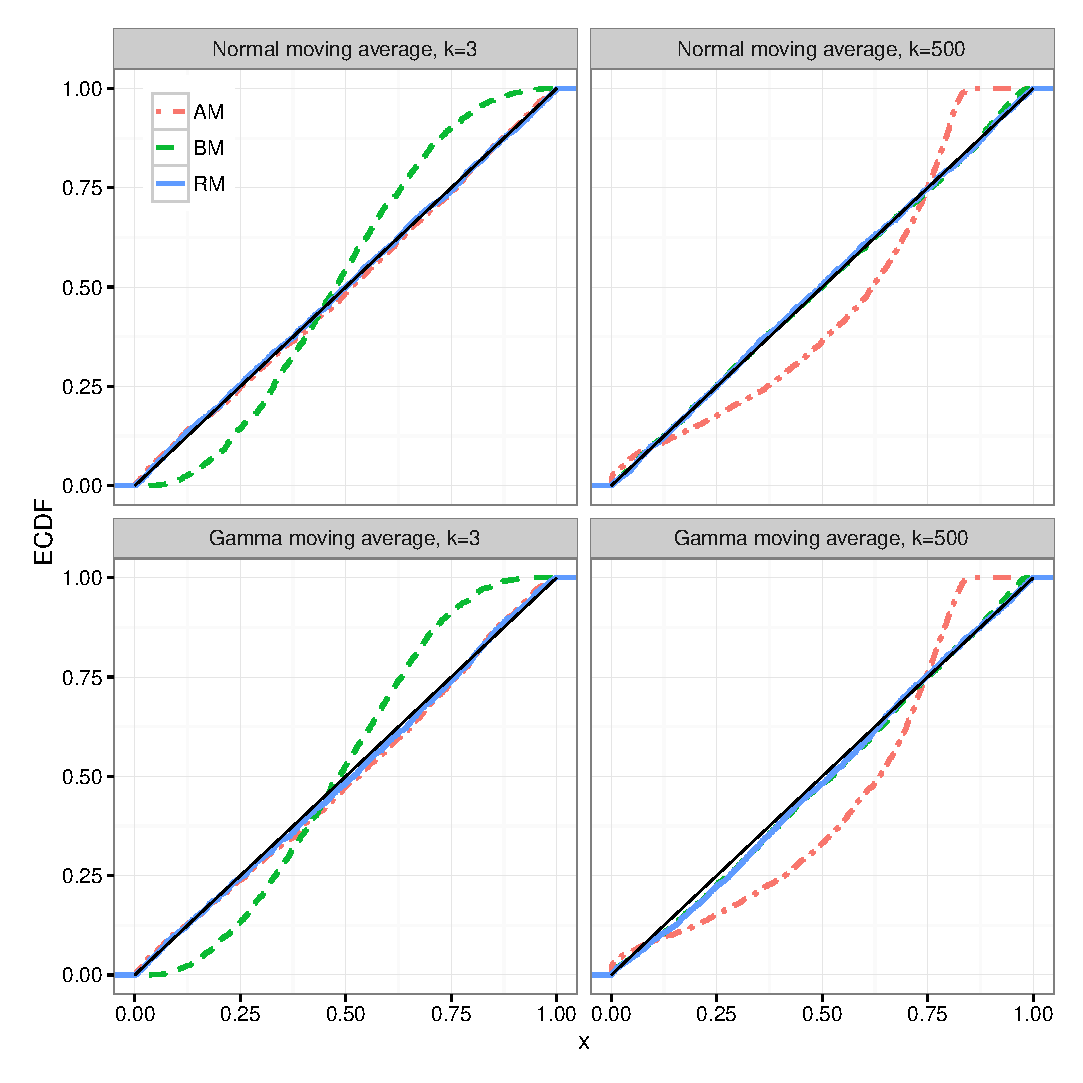
\includegraphics[ width=\textwidth]{Fig1}
    \caption{The ECDF of $2000$ independent $p$-values for the asymptotic method (AM), the bootstrap method (BM) and the randomization method (RM).  $p=600$, $n=100$.}\label{figure:ECDF}
\end{figure*}

%In Theorem~\ref{shaziCLT}, we showed that the randomization distribution tends to a standard normal distribution under certain conditions.
%In Figure~\ref{figure:histogram}, we plot the histograms of the randomization distribution under null hypothesis.
%For comparison, we also plot the standard normal density.
%From the plots, we can see that the randomization distribution is very similar to the standard normal distribution in factor model and moving average model with $k=3$.
%This verifies the Theorem~\ref{shaziCLT}.
%However, under moving average model with $k=500$, the randomization distribution is far from standard normal distribution.
%In fact, in this case, $\lambda_1(\Sigma)/\sqrt{\mytr(\Sigma^2)}$ is not negligible and~\eqref{chenC3} is not satisfied.
%This implies the accuracy of normal approximation depends on the innovation model.
%
%
%\begin{figure*}[htbp]
    %\centering
    %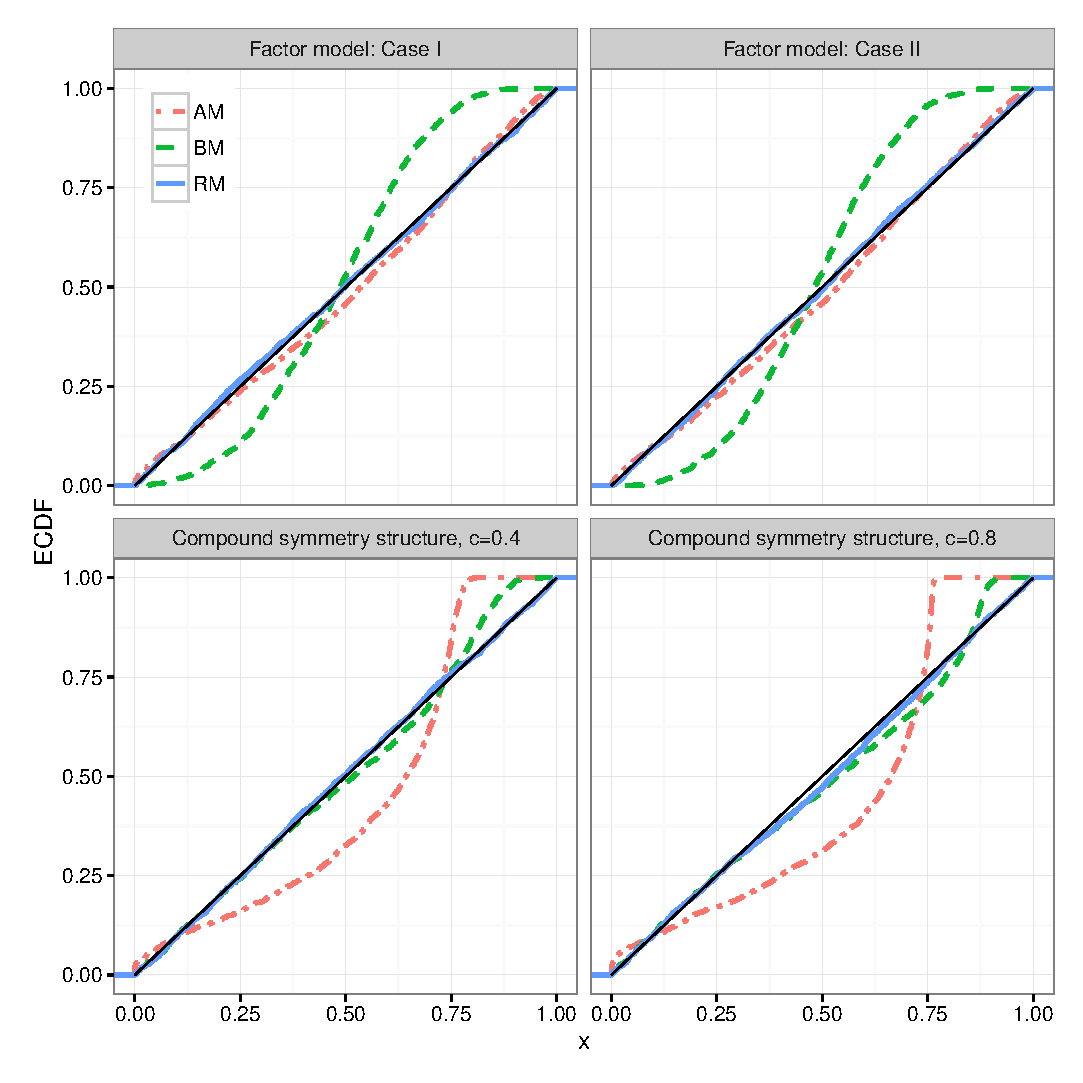
\includegraphics[width=0.48\textwidth]{Fig2}
    %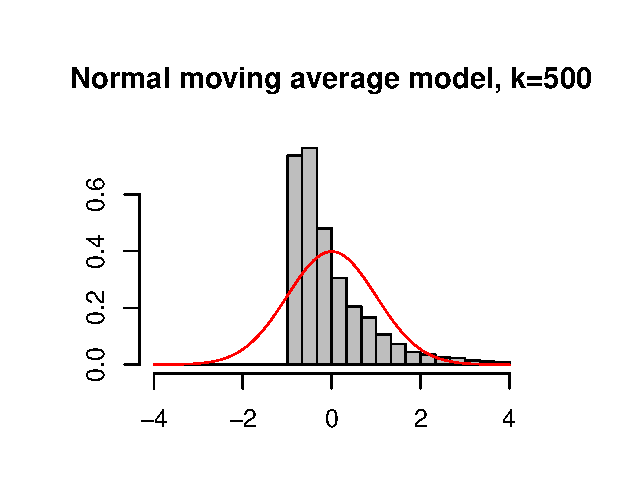
\includegraphics[width=0.48\textwidth]{Fig3}\\
    %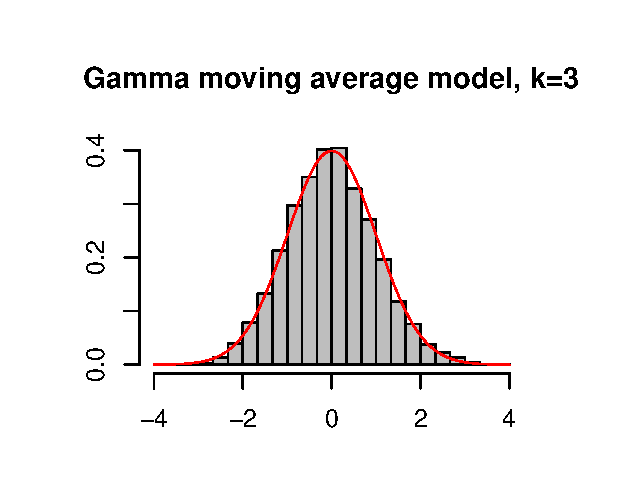
\includegraphics[width=0.48\textwidth]{Fig4}
    %\includegraphics[width=0.48\textwidth]{Fig5}\\
    %\includegraphics[width=0.48\textwidth]{Fig6}
    %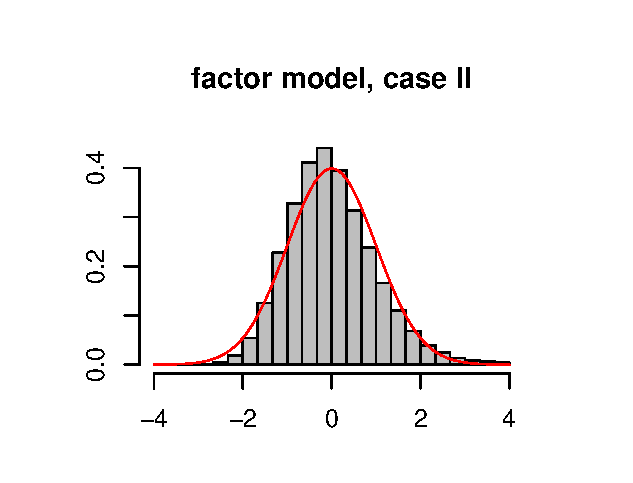
\includegraphics[width=0.48\textwidth]{Fig7}\\
    %\caption{The histograms of the randomization distribution. $p=600$, $n=100$.}\label{figure:histogram}
%\end{figure*}




Now we simulate the empirical power and size of the randomization test and the asymptotic method.
Let 
\begin{equation*}
    \mathrm{SNR}=\frac{\sqrt{n(n-1)}\mu^T \mu}{\sqrt{2\mytr \Sigma^2}}
\end{equation*}
be the signal to noise ratio (SNR).
%The theoretic asymptotic power is an increasing function of SNR\@.
We scale $\mu$ to reach different levels of SNR\@.
Our simulations consider two mean structure: dense mean and sparse mean.
In the dense mean setting,  we independently generate each coordinate of $\mu$ from $U(2,3)$ and then scale $\mu$ to reach a given SNR\@.
In the sparse mean setting, we randomly select $5\%$ of $\mu$'s $p$ coordinates to be non-zero.
Each non-zero coordinate is again independently generated from $U(2,3)$ and then scaled to reach a given SNR\@.
The empirical power and size are computed based on $2000$ simulations.
The nominal level $\alpha$ is $0.05$.

Table~\ref{table1} and Table~\ref{table2} list the empirical power and size for the moving average model.
It's not surprising that the randomization test can  control the Type I error rate well in normal case.
The results also show that the randomization method can control the Type I error rate well in gamma case even if gamma distribution is not symmetric under null.
It justifies the robustness of the randomization method.
{\color{red}
On the other hand, the asymptotic method has small size when the correlations between variables are weak and has inflated size when the correlations are strong.
}
The empirical power of the randomization method is similar to the asymptotic method.
%They are both similar to theoretical asymptotic power~\eqref{oPower} when $k$ is small and are both lower than theoretical asymptotic power when $k$ is large.
Table~\ref{table3} lists the empirical power and size under factor model.
Although the distribution is not symmetric, the results show that the level of the randomization method is close to nominal level while the asymptotic method suffers from level inflation.
In summary, the simulation results show that the randomization method is robust and has similar power with asymptotic method.

\begin{table*}[ht]
    \caption{Empirical power and size of moving average model with normal innovation. TP represents the theoretical asymptotic power, RM represents the randomization method, AM represents the asymptotic method.}
\label{table1}
    \centering
    \begin{tabular}{cclccccccccc}
          \toprule
          &&& & \multicolumn{4}{c}{Dense means} &\multicolumn{4}{c}{Sparse means}\\
          \cmidrule(r){5-8}\cmidrule(r){9-12}
          &&& & \multicolumn{2}{c}{$k=3$} & \multicolumn{2}{c}{$k=500$} & \multicolumn{2}{c}{$k=3$}& \multicolumn{2}{c}{$k=500$}\\
          \cmidrule(r){5-6}  \cmidrule(r){7-8} \cmidrule(r){9-10}  \cmidrule(r){11-12}
           $n$&$p$&SNR& TP & RM & AM & RM & AM & RM & AM & RM & AM  \\ 
            \midrule
        100&600&0.0 (size) & 0.050 & 0.0445 & 0.0515 & 0.0530 & 0.0745 & 0.0500 & 0.0585 & 0.0515 & 0.0715 \\ 
          &&0.5 & 0.126 & 0.1815 & 0.1940 & 0.1330 & 0.1685 & 0.1735 & 0.1875 & 0.0780 & 0.1130 \\ 
            &&1.0 & 0.260 & 0.4075 & 0.4295 & 0.2250 & 0.2785 & 0.4060 & 0.4325 & 0.1505 & 0.2065 \\ 
              &&1.5 & 0.442 & 0.6295 & 0.6535 & 0.3435 & 0.3920 & 0.6520 & 0.6755 & 0.2480 & 0.3355 \\ 
                &&2.0 & 0.639 & 0.7895 & 0.8055 & 0.3935 & 0.4665 & 0.8575 & 0.8765 & 0.3850 & 0.5400 \\ 
                  &&2.5 & 0.804 & 0.9165 & 0.9215 & 0.4775 & 0.5425 & 0.9655 & 0.9695 & 0.6355 & 0.8155 \\ 
                    &&3.0 & 0.912 & 0.9640 & 0.9695 & 0.5445 & 0.6090 & 0.9910 & 0.9935 & 0.8720 & 0.9730 \\ 
% new simulations
        \midrule
        200&1000&0.0 (size) & 0.050 & 0.0505 & 0.0550 & 0.0505 & 0.0695 & 0.0520 & 0.0575 & 0.0510 & 0.0700 \\ 
          &&0.5 & 0.126 & 0.1885 & 0.2025 & 0.1410 & 0.1680 & 0.1745 & 0.1865 & 0.0855 & 0.1165 \\ 
            &&1.0 & 0.260 & 0.3875 & 0.4050 & 0.2090 & 0.2620 & 0.4010 & 0.4160 & 0.1485 & 0.2075 \\ 
              &&1.5 & 0.442 & 0.6425 & 0.6600 & 0.3180 & 0.3715 & 0.6725 & 0.6895 & 0.2355 & 0.3290 \\ 
                &&2.0 & 0.639 & 0.8245 & 0.8355 & 0.4210 & 0.4760 & 0.8710 & 0.8845 & 0.3855 & 0.5310 \\ 
                  &&2.5 & 0.804 & 0.9210 & 0.9265 & 0.4885 & 0.5475 & 0.9690 & 0.9710 & 0.6290 & 0.8050 \\ 
                    &&3.0 & 0.912 & 0.9820 & 0.9830 & 0.6045 & 0.6530 & 0.9940 & 0.9960 & 0.8670 & 0.9780 \\ 
        \bottomrule
    \end{tabular}
\end{table*}

\begin{table*}[ht]
    \caption{Empirical power and size of moving average model with Gamma innovation.   TP is the theoretical asymptotic power, RM represents the randomization method, AM represents the asymptotic method.}
\label{table2}
    \centering
    \begin{tabular}{cclccccccccc}
          \toprule
          &&& & \multicolumn{4}{c}{Dense means} &\multicolumn{4}{c}{Sparse means}\\
          \cmidrule(r){5-8}\cmidrule(r){9-12}
          &&& & \multicolumn{2}{c}{$k=3$} & \multicolumn{2}{c}{$k=500$} & \multicolumn{2}{c}{$k=3$}& \multicolumn{2}{c}{$k=500$}\\
          \cmidrule(r){5-6}  \cmidrule(r){7-8} \cmidrule(r){9-10}  \cmidrule(r){11-12}
           $n$&$p$&SNR& TP & RM & AM & RM & AM & RM & AM & RM & AM \\ 
            \midrule
        100&600&0.0 (size) & 0.050 & 0.0450 & 0.0550 & 0.0475 & 0.0660 & 0.0405 & 0.0465 & 0.0505 & 0.0765 \\ 
          &&0.5 & 0.126 & 0.1815 & 0.1975 & 0.1365 & 0.1750 & 0.1765 & 0.1870 & 0.0985 & 0.1345 \\ 
            &&1.0 & 0.260 & 0.3825 & 0.4050 & 0.2375 & 0.2765 & 0.4130 & 0.4335 & 0.1550 & 0.2070 \\ 
              &&1.5 & 0.442 & 0.6210 & 0.6465 & 0.2975 & 0.3490 & 0.6580 & 0.6745 & 0.2225 & 0.3135 \\ 
                &&2.0 & 0.639 & 0.8180 & 0.8325 & 0.3920 & 0.4450 & 0.8645 & 0.8800 & 0.3890 & 0.5340 \\ 
                  &&2.5 & 0.804 & 0.9115 & 0.9260 & 0.4900 & 0.5465 & 0.9635 & 0.9665 & 0.6280 & 0.8200 \\ 
                    &&3.0 & 0.912 & 0.9710 & 0.9765 & 0.5505 & 0.6085 & 0.9940 & 0.9945 & 0.8600 & 0.9740 \\ 
% new simulation
        \midrule
                   200 & 1000 &0.0 (size) & 0.050 & 0.0520 & 0.0555 & 0.0495 & 0.0715 & 0.0505 & 0.0555 & 0.0455 & 0.0690 \\ 
                      &&0.5 & 0.126 & 0.1740 & 0.1880 & 0.1355 & 0.1725 & 0.1725 & 0.1840 & 0.0780 & 0.1170 \\ 
                        &&1.0 & 0.260 & 0.3890 & 0.4045 & 0.2175 & 0.2595 & 0.4220 & 0.4415 & 0.1475 & 0.1950 \\ 
                          &&1.5 & 0.442 & 0.6470 & 0.6630 & 0.3240 & 0.3820 & 0.6605 & 0.6855 & 0.2550 & 0.3375 \\ 
                            &&2.0 & 0.639 & 0.8175 & 0.8285 & 0.4180 & 0.4755 & 0.8580 & 0.8750 & 0.3835 & 0.5205 \\ 
                              &&2.5 & 0.804 & 0.9295 & 0.9335 & 0.4870 & 0.5560 & 0.9600 & 0.9645 & 0.6075 & 0.7970 \\ 
                                &&3.0 & 0.912 & 0.9755 & 0.9765 & 0.5865 & 0.6505 & 0.9915 & 0.9935 & 0.8760 & 0.9790 \\ 
        \bottomrule
    \end{tabular}
\end{table*}

\begin{table*}[ht]
    \caption{Empirical power and size of factor model innovation.  TP is the theoretical asymptotic power, RM represents the randomization method, AM represents the asymptotic method.}
\label{table3}
    \centering
    \begin{tabular}{cclccccccccc}
          \toprule
          &&& & \multicolumn{4}{c}{Dense means} &\multicolumn{4}{c}{Sparse means}\\
          \cmidrule(r){5-8}\cmidrule(r){9-12}
          &&& & \multicolumn{2}{c}{Case I} & \multicolumn{2}{c}{Case II} & \multicolumn{2}{c}{Case I}& \multicolumn{2}{c}{Case II}\\
          \cmidrule(r){5-6}  \cmidrule(r){7-8} \cmidrule(r){9-10}  \cmidrule(r){11-12}
           $n$&$p$&SNR& TP & RM & AM & RM & AM & RM & AM & RM & AM  \\ 
            \midrule
        100&600&0.0 (size) & 0.050 & 0.0465 & 0.0610 & 0.0455 & 0.0590 & 0.0475 & 0.0625 & 0.0505 & 0.0615 \\ 
          &&0.5 & 0.126 & 0.1315 & 0.1555 & 0.1465 & 0.1650 & 0.1200 & 0.1380 & 0.1080 & 0.1320 \\ 
            &&1.0 & 0.260 & 0.2420 & 0.2780 & 0.2550 & 0.2780 & 0.1940 & 0.2250 & 0.2075 & 0.2400 \\ 
              &&1.5 & 0.442 & 0.3635 & 0.3975 & 0.3555 & 0.3870 & 0.3670 & 0.4110 & 0.3740 & 0.4155 \\ 
                &&2.0 & 0.639 & 0.4825 & 0.5165 & 0.4720 & 0.4975 & 0.5340 & 0.5930 & 0.5615 & 0.6015 \\ 
                  &&2.5 & 0.804 & 0.5860 & 0.6190 & 0.5825 & 0.6165 & 0.7040 & 0.7610 & 0.7120 & 0.7505 \\ 
                    &&3.0 & 0.912 & 0.6730 & 0.7060 & 0.6975 & 0.7210 & 0.8525 & 0.8815 & 0.8680 & 0.8920 \\ 
        \midrule
        200&1002&0.0 (size) & 0.050 & 0.0520 & 0.0670 & 0.0530 & 0.0665 & 0.0485 & 0.0615 & 0.0490 & 0.0615 \\ 
          &&0.5 & 0.126 & 0.1490 & 0.1895 & 0.1405 & 0.1675 & 0.0905 & 0.1115 & 0.0975 & 0.1230 \\ 
            &&1.0 & 0.260 & 0.2450 & 0.2780 & 0.2485 & 0.2785 & 0.1835 & 0.2330 & 0.1920 & 0.2305 \\ 
              &&1.5 & 0.442 & 0.3445 & 0.3915 & 0.3450 & 0.3745 & 0.3170 & 0.3745 & 0.3395 & 0.3935 \\ 
                &&2.0 & 0.639 & 0.4605 & 0.5035 & 0.4775 & 0.5170 & 0.5080 & 0.5995 & 0.5365 & 0.5925 \\ 
                  &&2.5 & 0.804 & 0.5355 & 0.5810 & 0.5900 & 0.6320 & 0.7040 & 0.7775 & 0.7345 & 0.7850 \\ 
                    &&3.0 & 0.912 & 0.6280 & 0.6640 & 0.6660 & 0.6960 & 0.8670 & 0.9115 & 0.8655 & 0.9070 \\ 
        \bottomrule
    \end{tabular}
\end{table*}

%\subsection{The second simulation study}
%The computation of our randomization test is easy since we only need to compute $X_i^T X_j$ once, $1\leq j<i \leq n$.
%The same technique can be applied to the statistic $\sum_{i\neq j}\|X_i\|^{-1}\|X_j\|^{-1}X_i^T X_j$ in~\cite{Wang2015A}.
%However, the technique can not be applied to the statistic $\bar{X}^T [\mydiag(S)]^{-1}\bar{X}$ in~\cite{Srivastava2008A} and the statistic $\bar{X}^T (I_p-\BP_S)\bar{X}$ in~\cite{Zhao2016A}.
%Generally, many high dimensional test statistics for hypotheses~\eqref{ourHy} can be written as generalized quadratic forms of data
%$$
%\sum_{i=1}^n \sum_{j=1}^n X_i^T A X_j,
%$$
%Where $A$ is a $p\times p$ matrix which only depends on $S$.
%The difficulty is that for each randomization, the matrix $A$ should be recalculated.
%It consumes a lot time.
%However, 
%the matrix $A$ is used to estimate the structure of $\Sigma$, which should not change during randomization.
%This motivates us to hold $A$ constant during randomization.
%More precisely, for a randomization, we generate $\epsilon_1,\ldots,\epsilon_n$ and compute
%$$
%\sum_{j<i} X_i^T A X_j \epsilon_i \epsilon_j.
%$$
%We simulate the level.
%
%We consider the following $A$:
%$A_1=[\mydiag(S)]^{-1}$,
%$A_2=\bar{X} S^{+}\bar{X}$,
%$A_3=(I-\BP_S)$,
%$A_4=S$.







\section{Conclusion Remark}
In this paper, we considered a randomization test for mean vector in high dimensional setting.
A fast implementation was provided.
We also derived some asymptotic properties of the test procedure.
We showed that even if the symmetric assumption is violated, the randomization test also has correct level asymptotically.
Hence the test procedure is robust.
 In fact, the algorithm and the proof method can also be applied to other quadratic based statistics.
%It is interesting to investigate the robustness of randomization test in finite sample case.

In classical statistics, randomization test procedures are time consuming.
Nevertheless, the computational complexity of our randomization test procedure is not affected by the data dimension $p$. 
Hence we have reason to believe that randomization tests may be generally suitable for high dimensional problems.



Our randomization test can be immediately generalized to the two sample problem for paired data~\citep{Konietschke2014}.
However, maybe the most widely used randomization test for two sample problem is the permutation test.
As pointed by~\citet{Romano1990On}, the asymptotic property of randomization tests depends heavily on the particular problem and the randomization method.
The proof method used in this paper can not be applied to two sample permutation test.
 It is interesting to understand the behavior of permutation tests in high dimensional setting. We leave it for further work.


\section*{Acknowledgments}
{This work was supported by the National Natural Science Foundation of China under Grant No. 11471035, 11471030.
}

\appendix
\appendixpage
    
    Denote by $\Gamma^T \Gamma= Q\Lambda Q^T$ the spectral decomposition of $\Gamma^T \Gamma$, where  $Q$ is a $m\times p$ column orthogonal matrix and $\Lambda=\mydiag(\lambda_1(\Sigma),\ldots,\lambda_p(\Sigma))$.
    Let $\Lambda_{1}=\mydiag(\lambda_1(\Sigma),\ldots,\lambda_r(\Sigma))$, $\Lambda_{2}=\mydiag(\lambda_{r+1}(\Sigma),\ldots,\lambda_p(\Sigma))$.
    Write $Q=(Q_{1},Q_{2})$ where $Q_{1}$ and $Q_{2}$ are the first $r$ columns and last $p-r$ columns of $Q$ respectively.
    Then $\Gamma^T \Gamma=Q_1\Lambda_1 Q_1^T + Q_2 \Lambda_2 Q_2^T$.
For nonzero constants $c\in\mathbb{R}$ and $t\in\mathbb{R}^r$, we denote
$$
    Y_{ij}=\big(\frac{n(n-1)}{2} \mytr(\Sigma^2)\big)^{-1/2}Z_i^T Q_2 \Lambda_2 Q_2^T Z_j,
    \quad
    Y^*_i=n^{-1/2} Q_1^T Z_i.
$$

\section{Preparatory technical results}
We state in this section some technical results that are used in the proofs of the main results.

\begin{lemma}\label{lemmaUniformSimple}
    Suppose $\{\eta_n\}_{n=1}^{\infty}$ is a sequence of random variables, weakly converges to $\eta$, a random variable with continuous distribution function.
    Then we have
    \begin{equation*}
        \sup_{x\in\mathbb{R}}|\Pr(\eta_n\leq x)-\Pr(\eta\leq x)|\to 0.
    \end{equation*}
\end{lemma}


\begin{lemma}\label{lemma:zhong1}
    Under the condition~\eqref{chenC2}, we have
    \begin{enumerate}[(i)]
        \item
            for any $m\times m$ positive semidefinite matrix $B$,
            \begin{equation*}\label{zhong1}
            \myE(Z_1^T B Z_1)^2\leq (3+\Delta) \mytr^2(B),\quad
            \myVar(Z_1^T B Z_1)\leq (2+\Delta) \mytr(B^2);
            \end{equation*}
        %\item
            %for any $m\times m$ symmetric matrices $B_1$ and $B_2$,
            %\begin{equation}\label{zhong1}
            %\myE (Z_1^T B_1 Z_1)(Z_1^T B_2 Z_1)
            %=\mytr(B_1)\mytr(B_2)+2\mytr(B_1 B_2)+\Delta \mytr(B_1 \circ B_2);
            %\end{equation}
        \item
            for any $m\times m$ positive semidefinite matrix $B$,
            \begin{equation*}\label{zhong2}
                \myE (Z_1^T B Z_2)^4\leq (3+\Delta)^2\mytr^2 (B^2).
            \end{equation*}
    \end{enumerate}
\end{lemma}
\begin{proof}
    The inequality~\eqref{zhong1} follows from (i) of \citet[Proposition A.1]{songxi2010}.
    The inequality~\eqref{zhong2} is obtained by using~\eqref{zhong1} twice:
    $$
    \begin{aligned} 
        &\myE (Z_1^T B Z_2)^4
                =\myE\myE\big[ (Z_1^T B Z_2 Z_2^T B Z_1)^2|Z_2\big]
                \\
                \leq &
                (3+\Delta)\myE  \mytr^2 (B Z_2 Z_2^T B)
                =
                (3+\Delta)\myE  (Z_2^T B^2 Z_2 )^2
                \leq (3+\Delta)^2\mytr^2 (B^2).
    \end{aligned}
    $$

\end{proof}










\section{Proof of Theorem~\ref{prop:spiked1}}

\begin{proposition}\label{prop:spiked2}
    Under~\eqref{chenC1},~\eqref{chenC2},~\eqref{spikedC},
    we have
    $$
    \frac{\sum_{j<i} Z_i^T \Gamma^T \Gamma Z_j }
    {\sqrt{\frac{n(n-1)}{2}\mytr(\Sigma^2)}}
    \xrightarrow{w}\frac{\sqrt{2}}{2}\sum_{i=1}^r \kappa_i (\xi_i^2-1)+(1-\sum_{i=1}^r \kappa_i^2)^{1/2} \xi_{r+1},
    $$
    where $\xi_1,\ldots \xi_{r+1}$ are iid standard normal random variables.
\end{proposition}

\begin{proof}
    Note that
    $$
    \begin{aligned}
        &
    \frac{\sum_{j<i} Z_i^T \Gamma^T \Gamma Z_j }
    {\sqrt{\frac{n(n-1)}{2}\mytr(\Sigma^2)}}
        =
        \frac{\sum_{j<i}Z_i^T Q_1 \Lambda_1 Q_1^T Z_j}
    {\sqrt{\frac{n(n-1)}{2}\mytr(\Sigma^2)}}
        +
        \frac{\sum_{j<i}Z_i^T Q_2 \Lambda_2 Q_2^T Z_j}
    {\sqrt{\frac{n(n-1)}{2}\mytr(\Sigma^2)}}
    \\
        =&
        \big(2\frac{n-1}{n}\mytr(\Sigma^2)\big)^{-1/2}(\sum_{i=1}^n  Y_i^*)^T \Lambda_1 \sum_{i=1}^n  Y_i^*
        +
        \sum_{j<i} Y_{ij}
        -
        \big(2\frac{n-1}{n}\mytr(\Sigma^2)\big)^{-1/2}
        \sum_{i=1}^n Y_i^{*T}\Lambda_1 Y_i^*
        .
    \end{aligned}
    $$
    Next we show that 
    \begin{equation}\label{eq:toProveCLT}
        \big(
        (\sum_{i=1}^n Y_i^*)^T,
        \sum_{j<i} Y_{ij}
        \big)^T
    \xrightarrow{\mathcal{L}} N_{r+1}\Big(0_{r+1}, \mydiag \big(I_{r},1-\sum_{i=1}^r \kappa_i^2\big)\Big).
\end{equation}
    To prove this, it suffices to show that for any nonzero constants $t\in\mathbb{R}^r$ and $c\in\mathbb{R}$,
    \begin{equation}\label{eq:univariateCLT}
        t^T \sum_{i=1}^n Y_i^* +c \sum_{j<i} Y_{ij}
        \xrightarrow{\mathcal{L}}N\big(0,\|t\|^2+c^2(1-\sum_{i=1}^r \kappa_i^2)\big).
    \end{equation}
    Write $t^T \sum_{i=1}^n Y_i^*+c \sum_{j<i}Y_{ij} =\sum_{i=1}^n U_{in}$,
    where 
    $U_{in}=
    t^T Y_i^*+c  \sum_{j: j<i}Y_{ij}
    $.
    Let $\mathcal{F}_{in}$ be the $\sigma$-field generated by $X_1,\dots, X_i$, $k=1,\ldots,n$.
    Then $\{U_{in}\}_{i=1}^n$ is a martingale difference array with respect to $\{\mathcal{F}_{in}\}_{i=1}^n$.
    By the martingale central limit theorem~\citep[Chapter VIII, Theorem 1]{pollard1984convergence},~\eqref{eq:univariateCLT} holds provided
     \begin{equation}\label{eq:MCLTcondition1}
         \sum_{i=1}^n \myE(U_{in}^2 |\mathcal{F}_{i-1,n})\xrightarrow{P} \|t\|^2 + c^2(1-\sum_{i=1}^r \kappa_i^2),
     \end{equation}
     and for every $\epsilon>0$,
     \begin{equation}\label{eq:MCLTcondition2}
         \sum_{i=1}^n \myE\big(U_{in}^2\big\{U_{in}^2>\epsilon \big\}\big|\mathcal{F}_{i-1,n}\big)\xrightarrow{P} 0.
     \end{equation}
    We first verify~\eqref{eq:MCLTcondition1}. By direct calculation, we have
     $$
     \begin{aligned}
         &\sum_{i=1}^n \myE(U_{in}^2 |\mathcal{F}_{i-1,n})    
     =\|t\|^2+c^2 \big(\frac{n(n-1)}{2} \mytr(\Sigma^2)\big)^{-1}\sum_{i=1}^n \Big(\big(\sum_{j:j<i} Z_{j}\big)^T Q_2 \Lambda_2^2 Q_2^T \sum_{j:j<i} Z_{j}\Big).
     \end{aligned}
     $$
     Note that
     \begin{align}
         &\sum_{i=1}^n \Big(\big(\sum_{j:j<i} Z_{j}\big)^T Q_2 \Lambda_2^2 Q_2^T \sum_{j:j<i} Z_{j}\Big)
         =
    \sum_{i=1}^n \Big(
         \sum_{j:j<i} Z_{j}^T Q_2 \Lambda_2^2 Q_2^T  Z_{j}
         +
         2\sum_{j,k:k<j<i}Z_{j}^T Q_2 \Lambda_2^2 Q_2^T  Z_{k}
         \Big)
         \notag
         \\
         =&
         \sum_{j=1}^{n} (n-j) Z_{j}^T Q_2 \Lambda_2^2 Q_2^T  Z_{j}
         +
         2\sum_{k<j} (n-j) Z_{j}^T Q_2 \Lambda_2^2 Q_2^T  Z_{k}
         .
         \label{eq:shiwu}
     \end{align}
     The first term satisfies
     $$
     \begin{aligned}
\myE\sum_{j=1}^{n} (n-j) Z_{j}^T Q_2 \Lambda_2^2 Q_2^T  Z_{j}=
         \frac{n(n-1)}{2}\mytr (\Lambda_2^2)
     \end{aligned}
     $$
     and
     $$
     \begin{aligned}
         &\myVar\Big(\sum_{j=1}^{n} (n-j) Z_{j}^T Q_2 \Lambda_2^2 Q_2^T  Z_{j}\Big)=
         \frac{(n-1)n(2n-1)}{6}
         \myVar\big( Z_{1}^T Q_2 \Lambda_2^2 Q_2^T  Z_{1}\big)
         \leq (2+\Delta)
         n^3\mytr(\Lambda_2^4),
     \end{aligned}
     $$
     where the last inequality follows from (i) of Lemma~\ref{lemma:zhong1}.
     Hence
     \begin{equation}\label{eq:shiwu2}
     \begin{aligned}
         &
         {\sum_{j=1}^{n} (n-j) Z_{j}^T Q_2 \Lambda_2^2 Q_2^T  Z_{j}}
         =
         \frac{n(n-1)}{2}\mytr(\Lambda_2^2)+O_{P}\big(n^{3/2} \mytr^{1/2} (\Lambda_2^4)\big)
         \\
         =&
\big(\frac{n(n-1)}{2}\mytr (\Sigma^2)\big)
         \Big(\frac{\mytr (\Lambda_2^2)}{\mytr(\Sigma^2)} +o_P(1)\Big)
         =
\big(\frac{n(n-1)}{2}\mytr (\Sigma^2)\big)
         \Big(1-\sum_{i=1}^r \kappa_i^2 +o_P(1)\Big).
     \end{aligned}
     \end{equation}
     As for the second term of~\eqref{eq:shiwu}, we have
     $$
     \begin{aligned}
         &\myE \big(
    \sum_{k<j} (n-j)Z_j^T Q_2 \Lambda_2^2 Q_2^T Z_k 
     \big)^2
     =
    \sum_{k<j} (n-j)^2 \myE \big(Z_j^T Q_2 \Lambda_2^2 Q_2^T Z_k 
     \big)^2
         =
  \sum_{k<j} (n-j)^2 \mytr(\Lambda_2^4)\\
         \leq & n^4\mytr(\Lambda_2^4) 
         \leq  n^4 \lambda_{r+1}^2(\Sigma)\mytr(\Lambda_2^2)
         =
         o\Big(\big(\frac{n(n-1)}{2}\mytr (\Sigma^2)\big)^2\Big)
         .
     \end{aligned}
     $$
     Hence
     \begin{equation}\label{eq:shiwu3}
     \begin{aligned}
    \sum_{k<j} (n-j)Z_j^T Q_2 \Lambda_2^2 Q_2^T Z_k 
         =
         o_P\big(\frac{n(n-1)}{2}\mytr (\Sigma^2)\big)
         .
     \end{aligned}
     \end{equation}
         Combining~\eqref{eq:shiwu},~\eqref{eq:shiwu2} and~\eqref{eq:shiwu3} yields
     $$
         \big(\frac{n(n-1)}{2}\mytr (\Sigma^2)\big)^{-1} \sum_{i=1}^n \Big(\big(\sum_{j:j<i} Z_{j}\big)^T Q_2 \Lambda_2^2 Q_2^T \sum_{j:j<i} Z_{j}\Big)
         = 1-\sum_{i=1}^r \kappa_i^2+o_P(1).
     $$
     This proves~\eqref{eq:MCLTcondition1}.
     
     Now we verify~\eqref{eq:MCLTcondition2}.
     By Markov's inequality, it suffices to show $\sum_{i=1}^n \myE\big(U_{in}^4\big)\to 0$.
     Note that
     $$
     \begin{aligned}
         &\myE\big(U_{in}^4\big)
         \leq
         8n^{-2}\myE \big(t^T Q_1^T Z_i\big)^4+
         8c^2  
         \big(\frac{n(n-1)}{2} \mytr(\Sigma^2)\big)^{-2}
         \myE\big( Z_i^T Q_2 \Lambda_2 Q_2^T \sum_{j:j<i}Z_j\big)^4.
     \end{aligned}
     $$
    Applying (i) of Lemma~\ref{lemma:zhong1} yields
    $$
\myE \big(t^T Q_1^T Z_i\big)^4\leq
         \myE \big( Z_i^T Q_1 t t^T Q_1^T Z_i\big)^2
         \leq (3+\Delta)\mytr^2 (Q_1 t t^T Q_1^T)
         = (3+\Delta) \|t\|^4.
    $$
    Also by (i) of Lemma~\ref{lemma:zhong1},
    $$
    \begin{aligned}
        &
         \myE\big( Z_i^T Q_2 \Lambda_2 Q_2^T \sum_{j:j<i}Z_j\big)^4
         =
        \myE\big( Z_i^T Q_2 \Lambda_2 Q_2^T (\sum_{j:j<i}Z_j)(\sum_{j:j<i}Z_j)^T Q_2 \Lambda_2 Q_2^T Z_i\big)^2
        \\
        \leq &
        (3+\Delta)\myE \mytr^2 (Q_2 \Lambda_2 Q_2^T (\sum_{j:j<i}Z_j)(\sum_{j:j<i}Z_j)^T Q_2 \Lambda_2 Q_2^T)
        \\
        = &
        (3+\Delta)\myE  \Big((\sum_{j:j<i}Z_j)^T Q_2 \Lambda_2^2 Q_2^T (\sum_{j:j<i}Z_j)\Big)^2
        \\
        = &
        (3+\Delta)\myE  \Big(\sum_{j:j<i}Z_j^T Q_2 \Lambda_2^2 Q_2^T Z_j+2\sum_{j,k:k<j<i}Z_j^T Q_2 \Lambda_2^2 Q_2^T Z_k\Big)^2
        \\
        = &
        (3+\Delta)\myE  \Big(\sum_{j:j<i}Z_j^T Q_2 \Lambda_2^2 Q_2^T Z_j \Big)^2+4(3+\Delta)\myE \Big(\sum_{j,k:k<j<i}Z_j^T Q_2 \Lambda_2^2 Q_2^T Z_k\Big)^2
        \\
        \leq &
        (3+\Delta)^2 (i-1)^2 \mytr^2 (\Lambda_2^2)  +2(3+\Delta)(i-1)(i-2)\mytr(\Lambda_2^4)
        \\
        \leq &
        2(3+\Delta)^2 i^2 \mytr^2 (\Lambda_2^2).
    \end{aligned}
    $$
    Thus,
     $$
         \myE\big(U_{in}^4\big)
         \leq 8 (3+\Delta)\|t\|^4 n^{-2}+
         16 c^2 (3+\Delta)^2 i^2 \big(\frac{n(n-1)}{2}\big)^{-2}.
     $$
     It follows that
     $
         \sum_{i=1}^n \myE\big(U_{in}^4\big)
        \to 0.
     $
     This completes the proof of~\eqref{eq:toProveCLT}.

    

    It follows from~\eqref{eq:toProveCLT} and Slutsky's theorem that
    $$
    \begin{aligned}
        &\big(2\frac{n-1}{n}\mytr(\Sigma^2)\big)^{-1/2}(\sum_{i=1}^n  Y_i^*)^T \Lambda_1 \sum_{i=1}^n  Y_i^*
        +
        \sum_{j<i} Y_{ij}
        \xrightarrow{w} \frac{\sqrt{2}}{2}\sum_{i=1}^r \kappa_i \xi_i^2+ (1-\sum_{i=1}^r \kappa_i^2)^{1/2}\xi_{r+1}.
    \end{aligned}
    $$
    It remains to show that
        $$
        \big(2\frac{n-1}{n}\mytr(\Sigma^2)\big)^{-1/2}
        \sum_{i=1}^n Y_i^{*T}\Lambda_1 Y_i^*
      \xrightarrow{P}\frac{\sqrt{2}}{2}\sum_{i=1}^r \kappa_i.
        $$
        This follows from
        $$
        \begin{aligned}
            &\myE
        \big(2\frac{n-1}{n}\mytr(\Sigma^2)\big)^{-1/2}
        \sum_{i=1}^n Y_i^{*T}\Lambda_1 Y_i^*
            =
        \big(2\frac{n-1}{n}\mytr(\Sigma^2)\big)^{-1/2}\mytr(\Lambda_1)
            =\frac{\sqrt{2}}{2}\sum_{i=1}^r \kappa_i+o(1)
        \end{aligned}
        $$
        and
        $$
        \begin{aligned}
            &\myVar\Big(
        \big(2\frac{n-1}{n}\mytr(\Sigma^2)\big)^{-1/2}
        \sum_{i=1}^n Y_i^{*T}\Lambda_1 Y_i^*
            \Big)
            =\big(2\frac{n-1}{n}\mytr(\Sigma^2)\big)^{-1} \frac{(2+\Delta)\mytr(\Lambda_1^2)}{n}=o(1).
        \end{aligned}
        $$
        This completes the proof.
    
\end{proof}


\begin{proof}[\textbf{Proof of Theorem~\ref{prop:spiked1}}]
    Note that
    \begin{equation}\label{eq:deco}
        {T(X_1,\ldots,X_n)-\frac{n(n-1)}{2}\|\mu\|^2}
        %{\sqrt{\frac{n(n-1)}{2}\mytr(\Sigma^2)}}
    =
        {\sum_{j<i} Z_i^T \Gamma^T \Gamma Z_j}
        %{\sqrt{\frac{n(n-1)}{2}\mytr(\Sigma^2)}}
    +
        {(n-1) \sum_{i=1}^n \mu^T \Gamma Z_i}.
        %{\sqrt{\frac{n(n-1)}{2}\mytr(\Sigma^2)}}.
    \end{equation}
    By central limit theorem,
        \begin{equation}\label{eq:aqiu}
        \frac{ \sum_{i=1}^n \mu^T \Gamma Z_i}
        {\sqrt{n\mu^T \Sigma \mu}}
        \xrightarrow{\mathcal{L}}N(0,1).
        \end{equation}
    If $\mu^T \Sigma \mu=o(n^{-1}\mytr(\Sigma^2))$, the first term of~\eqref{eq:deco} dominates the second term of~\eqref{eq:deco}, and the theorem follows from Proposition~\ref{prop:spiked2}.
    On the other hand, if $n^{-1}\mytr(\Sigma^2)=o(\mu^T \Sigma \mu)$, the second term of~\eqref{eq:deco} dominates the first term of~\eqref{eq:deco}, and the theorem follows from~\eqref{eq:aqiu}.



\end{proof}







\section{Proof of Theorem~\ref{ourTheorem}}

\paragraph{A central limit theorem for quadratic form of Rademacher variables}
The proof of the Theorem~\ref{shaziCLT} is based on a central limit theorem of the quadratic form of Rademacher variables. 
Such a central limit theorem can be also used to study the asymptotic behavior of many other randomization test.
 Let $\epsilon_1,\ldots,\epsilon_n$ be independent Rademacher  variables. 
 Consider the quadratic form $W_n=\sum_{1\leq j<i\leq n} a_{ij}\epsilon_i \epsilon_j+\sum_{i=1}^n b_i \epsilon_i$, where $\{a_{ij}\}_{1\leq j <i \leq n}$ and $\{b_i\}_{1\leq i\leq n}$ are nonrandom numbers.
 Here $\{\epsilon_i\}$, $\{a_{ij}\}$ and $\{b_{i}\}$ may depend on $n$, a parameter we suppress.
 By direct calculation, we have $\myE(W_n)=0$ and $\mathrm{Var}(W_n)=\sum_{1\leq j<i\leq n} a_{ij}^2+\sum_{i=1}^n b_i^2$.

 \begin{proposition}\label{CLTprop}
     A sufficient condition for
     \begin{equation*}
         \frac{W_n}{\sqrt{\sum_{1\leq j<i\leq n} a_{ij}^2 +\sum_{i=1}^n b_i^2}}
         \xrightarrow{\mathcal{L}} N(0,1)
     \end{equation*}
     is that
     \begin{equation}\label{complC}
         \sum_{k<j}{(\sum_{i:i>j}a_{ij}a_{ik})}^2+
         \sum_{j<i}a_{ij}^4+
         \sum_{k<j<i}a_{ij}^2 a_{ik}^2
         +
     \sum_{j=1}^n (\sum_{i:i>j} a_{ij}b_i)^2 
         +
         \sum_{i=1}^n b_i^4
         =o\Big(\big(\sum_{j<i} a_{ij}^2+\sum_{i=1}^n b_i^2\big)^2\Big).
     \end{equation}
 \end{proposition}

 \begin{proof}
     Note that we have the decomposition $W_n=\sum_{i=1}^n U_{in}$, where $U_{in} =\epsilon_i (\sum_{j:j<i} a_{ij}\epsilon_j+b_i )$, $i=1,\ldots,n$.
    Let $\mathcal{F}_{in}$ be the $\sigma$-field generated by $\epsilon_1,\ldots,\epsilon_i$, $i=1,\ldots, n$.
     Then $\{U_{in}\}_{i=1}^n$ is a martingale difference array with respect to $\{\mathcal{F}_{in}\}_{i=1}^n$. 
     By the martingale central limit theorem~\citep[Theorem 1 of Chapter VIII ]{pollard1984convergence}, the conclusion holds if the following two conditions are satisfied:
     \begin{equation}\label{MCLTcondition1}
         \frac{\sum_{i=2}^n \myE(U_{in}^2 |\mathcal{F}_{i-1,n})}{\sum_{j<i} a_{ij}^2+\sum_{i=1}^n b_i^2}\xrightarrow{P} 1,
     \end{equation}
     and
     \begin{equation}\label{MCLTcondition2}
         \frac{\sum_{i=2}^n \myE\big(U_{in}^2\big\{U_{in}^2>\epsilon (\sum_{j<i} a_{ij}^2+\sum_{i=1}^n b_i^2)\big\}\big|\mathcal{F}_{i-1,n}\big)}{\sum_{ j<i} a_{ij}^2+\sum_{i=1}^n b_i^2}\xrightarrow{P} 0,
     \end{equation}
     for every $\epsilon>0$.

     \paragraph{Proof of~\eqref{MCLTcondition1}}
By direct calculation, we have
     \begin{equation*}
         \begin{aligned}
             &\sum_{i=1}^n \myE(U_{in}^2 |\mathcal{F}_{i-1,n})
             =\sum_{i=1}^n \big(\sum_{j:j<i}a_{ij}\epsilon_j +b_i \big)^2\\
             %=&\sum_{i=1}^n \big( \sum_{j=1}^{i-1} a_{ij}^2 +2\sum_{j,k:j<k<i} a_{ij}a_{ik}\epsilon_j \epsilon_k + 2b_i\sum_{j=1}^{i-1}a_{ij}\epsilon_j + b_i^2\big)\\
             =&\sum_{j<i} a_{ij}^2+\sum_{i=1}^n b_i^2 +2\sum_{k<j} \sum_{i:i>j}(a_{ij}a_{ik})\epsilon_j \epsilon_k+2\sum_{j=1}^n (\sum_{i:i>j} a_{ij}b_i) \epsilon_j.
         \end{aligned}
     \end{equation*}
     By assumption, we have
     \begin{equation*}
         \begin{aligned}
             \myE{\big(\sum_{k<j} (\sum_{i:i>j}a_{ij}a_{ik})\epsilon_j \epsilon_k \big)}^2
             =
             \sum_{k<j} (\sum_{i:i>j}a_{ij}a_{ik})^2
             =
             o\big((\sum_{j<i} a_{ij}^2 +\sum_{i=1}^n b_i^2)^2\big)
         \end{aligned}
     \end{equation*}
     and
     $$
     \myE \big(\sum_{j=1}^n (\sum_{i:i>j} a_{ij}b_i) \epsilon_j\big)^2
     =
     \sum_{j=1}^n (\sum_{i:i>j} a_{ij}b_i)^2 
             =
             o\big((\sum_{j<i} a_{ij}^2 +\sum_{i=1}^n b_i^2)^2\big)
     $$
     Hence~\eqref{MCLTcondition1} holds.
     \paragraph{Proof of~\eqref{MCLTcondition2}}
     By Markov inequality, it's sufficient to prove
     \begin{equation}\label{temp1}
         \frac{\sum_{i=1}^n \myE\big(U_{in}^4\big|\mathcal{F}_{i-1,n}\big)}{{\big(\sum_{j<i} a_{ij}^2+\sum_{i=1}^n b_i^2\big)}^2}\xrightarrow{P} 0.
     \end{equation}
     Since the relevant random variables are all positive, we only need to prove~\eqref{temp1} converges to $0$ in mean. But
     \begin{equation*}
         \begin{aligned}
             &\sum_{i=1}^n \myE U_{in}^4
             =
             \sum_{i=1}^n \myE (\sum_{j:j<i}a_{ij}\epsilon_j+b_i)^4
             \leq
             8\sum_{i=1}^n \myE (\sum_{j:j<i}a_{ij}\epsilon_j)^4
             +8\sum_{i=1}^n b_i^4.
         \end{aligned}
     \end{equation*}
     By assumption, we have
     $$
     \sum_{i=1}^n b_i^4=
             o\Big(\big(\sum_{j<i} a_{ij}^2 +\sum_{i=1}^n b_i^2\big)^2\Big)
     $$
     and
     \begin{equation*}
         \begin{aligned}
             &\sum_{i=1}^n \myE (\sum_{j:j<i}a_{ij}\epsilon_j)^4=
             \sum_{i=1}^n \myE \big(\sum_{j:j<i}a_{ij}^2+2\sum_{j,k:k<j<i}a_{ij}a_{ik}\epsilon_j \epsilon_k \big)^2\\
             =&
             \sum_{i=1}^n  \big((\sum_{j:j<i}a_{ij}^2)^2+4\myE(\sum_{j,k:k<j<i}a_{ij}a_{ik}\epsilon_j \epsilon_k)^2 \big)
             =
             \sum_{i=1}^n  (\sum_{j:j<i}a_{ij}^4+6\sum_{j,k:k<j<i}a_{ij}^2 a_{ik}^2)\\
             =&
             \sum_{j<i}a_{ij}^4+6\sum_{k<j<i}a_{ij}^2 a_{ik}^2
             =
             o\Big(\big(\sum_{j<i} a_{ij}^2 +\sum_{i=1}^n b_i^2\big)^2\Big).
         \end{aligned}
     \end{equation*}
      Hence~\eqref{MCLTcondition2} holds.
      This completes the proof.
 \end{proof}

\begin{proposition}\label{proposition:jxz}
    Suppose~\eqref{chenC2} and~\eqref{spikedC} holds.
    %Let
%$$
    %a_{ij}=c\big(\frac{n(n-1)}{2} \mytr(\Sigma^2)\big)^{-1/2}Z_i^T Q_2 \Lambda_2 Q_2^T Z_j,
    %\quad
    %b_i=n^{-1/2} t^T Q_1^T Z_i.
%$$
    For nonzero constants $c\in\mathbb{R}$ and $t\in\mathbb{R}^r$,
    we have
    \begin{align}
    \label{lemma2R1}
        &\sum_{k<j}(\sum_{i:i>j}Y_{ij} Y_{ik})^2
        +\sum_{j<i}Y_{ij}^4
        +\sum_{k<j<i}Y_{ij}^2 Y_{ik}^2
        +\sum_{j=1}^n \big(\sum_{i:i>j} Y_{ij}t^T Y_i^*\big)^2
        +\sum_{i=1}^n (t^T Y_i^*)^4 \xrightarrow{P}0,
        \\
        &c^2 \sum_{j<i}Y_{ij}^2+\sum_{i=1}^n (t^T Y_i^*)^2=c^2(1-\sum_{i=1}^r \kappa_i^2)+\|t\|^2+o_P(1).\label{lemma2Rn}
    \end{align}
\end{proposition}
\begin{proof}
To prove~\eqref{lemma2R1}, we only need to show that the left hand side of~\eqref{lemma2R1} converges to $0$ in mean.
    For the first three terms of~\eqref{lemma2R1}, we have
    \begin{equation*}
    \begin{aligned}
        &\myE\sum_{k<j}\big(\sum_{i:i>j} Y_{ij} Y_{ik}\big)^2
        +\myE\sum_{j<i}Y_{ij}^4
        +\myE\sum_{k<j<i}Y_{ij}^2 Y_{ik}^2
        \\
        =&
        \myE\sum_{k<j}\Big(\sum_{i:i>j} Y_{ij}^2 Y_{ik}^2
        +2\sum_{i_1,i_2:i_1>i_2>j} Y_{i_1 j} Y_{i_1 k} Y_{i_2 j} Y_{i_2 k}\Big)
        +\myE\sum_{j<i}Y_{ij}^4
        +\myE\sum_{k<j<i}Y_{ij}^2 Y_{ik}^2
        \\
        =&
        2\myE\sum_{k<j<i_2<i_1}Y_{i_1 j} Y_{i_1 k} Y_{i_2 j} Y_{i_2 k}
        +2\myE\sum_{k<j<i}Y_{ij}^2 Y_{ik}^2
        +\myE\sum_{j<i}Y_{ij}^4
        \\
        =&
        \frac{(n-2)(n-3) \mytr(\Lambda_2^4)}{3n(n-1)\mytr^2(\Sigma^2)}
        +\frac{n(n-1)(n-2)}{3}\myE (Y_{31}^2 Y_{32}^2)
        +\frac{n(n-1)}{2}\myE Y_{21}^4
        \\
        \leq &
        \frac{(n-2)(n-3) \mytr(\Lambda_2^4)}{3n(n-1)\mytr^2(\Sigma^2)}
        +\Big(\frac{n(n-1)(n-2)}{3} +\frac{n(n-1)}{2}\Big)\myE Y_{21}^4
        \\
        \leq &
        \frac{(n-2)(n-3) \lambda_{r+1}(\Sigma)\mytr(\Lambda_2^2)}{3n(n-1)\mytr^2(\Sigma^2)}
        +\Big(\frac{n(n-1)(n-2)}{3} +\frac{n(n-1)}{2}\Big)
\frac{4(3+\Delta)^2\mytr^2(\Lambda_2^2)}{n^2(n-1)^2\mytr^2(\Sigma^2)}
        \to  0,
    \end{aligned}
    \end{equation*}
    where the last inequality follows from (ii) of Lemma~\ref{lemma:zhong1}.
    As for the fourth term of~\eqref{lemma2R1}, we have
$$
\begin{aligned}
    &\myE\sum_{j=1}^n \big(\sum_{i:i>j} Y_{ij} t^T Y_i^*\big)^2
=
    \myE\sum_{j<i} Y_{ij}^2 (t^T Y_i^{*})^2
    =
    \frac{n(n-1)}{2} \myE Y_{21}^2 (t^T Y_2^{*})^2
    \\
    =&
    \frac{n(n-1)}{2}  
    \myE \myE\big(Y_{21}^2 (t^T Y_2^{*})^2\big| Z_2\big)
    =\big(n\mytr(\Sigma^2)\big)^{-1} \myE \big( Z_2^T Q_2 \Lambda_2^2 Q_2^T Z_2 Z_2^T Q_1 t t^T Q_1^T Z_2\big) \\
    \leq&
    \big( n \mytr(\Sigma^2)\big)^{-1} 
    \big(\myE (Z_2^T Q_2 \Lambda_2^2 Q_2^T Z_2)^2\big)^{1/2} \big(\myE(Z_2^T Q_1 t t^T Q_1^T Z_2)^2\big)^{1/2}\\
    \leq&
     \frac{(3+\Delta) \|t\|^2}{n} 
    \frac{\mytr (\Lambda_2^2)}{\mytr(\Sigma^2)}\to 0,
\end{aligned}
$$
    where the last inequality follows from (i) of Lemma~\ref{lemma:zhong1}. 
    The last term of~\eqref{lemma2R1} satifies 
$$
        \myE\sum_{i=1}^n (t^T Y_i^*)^4=n \myE (t^T Y_i^*)^4
=\frac{1}{n} \myE (Z_1^T Q_1 t t^T Q_1^T Z_1)^2
\leq \frac{(3+\Delta)\|t\|^4}{n}\to 0.
$$
This completes the proof of~\eqref{lemma2R1}.



To prove~\eqref{lemma2Rn}, we show that
\begin{align}
    \sum_{j<i} Y_{ij}^2&= (1-\sum_{i=1}^r \kappa_i^2)+o_P(1),
    \label{eq:lemma2:1}
    \\
    \sum_{i=1}^n (t^T Y_i^*)^2&=\|t\|^2 +o_P(1).
    \label{eq:lemma2:2}
\end{align}
To prove~\eqref{eq:lemma2:1}, note that
$$
    \myE \big(\sum_{j<i} Y_{ij}^2\big)= \frac{\mytr(\Lambda_2^2)}{\mytr(\Sigma^2)}=(1-\sum_{i=1}^r \kappa_i^2)+o(1).
$$
    Hence we only need to show $\myVar\big(\sum_{j<i} Y_{ij}^2)=o(1)$. 
    Write $\big(\sum_{j<i}Y_{ij}^2\big)^2=
        \big(\sum_{j<i}Y_{ij}^2\big)
        \big(\sum_{l<k}Y_{kl}^2\big)$.
    Collect terms according to $\mathrm{card}(\{i,j\}\cap\{k,l\})=0,1,2$, we have
    \begin{equation*}%\label{eq:1}
    \begin{aligned}
        \big(\sum_{j<i}Y_{ij}^2\big)^2
        =&
        \sum_{j<i,l<k:\{i,j\}\cap \{k,l\}=\phi}Y_{ij}^2 Y_{kl}^2
        +2\sum_{j<i<k}\Big(
        Y_{ij}^2 Y_{ki}^2+
        Y_{ij}^2 Y_{kj}^2
        +
        Y_{kj}^2 Y_{ki}^2
        \Big)
         +
        \sum_{j<i}Y_{ij}^4.
    \end{aligned}
    \end{equation*}
    %For the three summations on the right hand side of equation~\eqref{eq:1},
    There are  $n(n-1)(n-2)(n-3)/4$, $n(n-1)(n-2)/6$ and $n(n-1)/2$ terms in each sum, respectively.
    For distinct $i,j,k,l$, 
    $$\myE Y_{ij}^2 Y_{kl}^2=(\myE Y_{12}^2)^2=\frac{4\mytr^2(\Lambda_2^2)}{n^2(n-1)^2\mytr^2(\Sigma^2)}.$$
    Otherwise, if $\text{card}(\{i,j\},\{k,l\})\geq 1$, by (ii) of Lemma~\ref{lemma:zhong1},
    $$\myE Y_{ij}^2 Y_{kl}^2\leq \myE Y_{12}^4\leq \frac{4(3+\Delta)^2\mytr^2(\Lambda_2^2)}{n^2(n-1)^2\mytr^2(\Sigma^2)}.$$
    Thus,
    \begin{equation*}
    \begin{aligned}
        \myE\big(\sum_{j<i}Y_{ij}^2\big)^2
            =& \frac{(n-2)(n-3)}{n(n-1)}\frac{\mytr^2 (\Lambda_2^2)}{\mytr^2(\Sigma^2)}
            +
            O(1)\big(n(n-1)(n-2)+\frac{n(n-1)}{2}\big)\frac{4(3+\Delta)^2\mytr^2(\Lambda_2^2)}{n^2(n-1)^2\mytr^2(\Sigma^2)}\\
            =& (1-\sum_{i=1}^r \kappa_i^2)^2+o(1).
    \end{aligned}
    \end{equation*}
    It follows that
    $
    \myVar\big(\sum_{j<i}Y_{ij}^2\big)=
    \myE\big(\sum_{j<i}Y_{ij}^2\big)^2-
    \big(\myE\sum_{j<i}Y_{ij}^2\big)^2=o(1)
    $, which completes the proof of~\eqref{eq:lemma2:1}.


    Finally, \eqref{eq:lemma2:2} follows from
$
\myE \big(\sum_{i=1}^n b_i^2\big)=\|t\|^2
$
and
$$
\myVar \big(\sum_{i=1}^n b_i^2 \big)=\frac{1}{n}\myVar (Z_1^T Q_1 t t^T Q_1^T Z_1)
\leq \frac{1}{n}(2+\Delta)\|t\|^4\to 0,
$$
where the last inequality follows from (i) of Lemma~\ref{lemma:zhong1}.
This completes the proof.


\end{proof}




\begin{proposition}\label{nomuProp}
    Under~\eqref{chenC1},~\eqref{chenC2},~\eqref{spikedC},
    we have
    $$
        \rho\Big(
        \mathcal{L}\Big(
    \frac{\sum_{j<i} Z_i^T \Gamma^T \Gamma Z_j \epsilon_i \epsilon_j}
    {\sqrt{\frac{n(n-1)}{2}\mytr(\Sigma^2)}}
        \Big|Z_1,\ldots,Z_n\Big)
        ,
        \mathcal{L}\big(\frac{\sqrt{2}}{2}\sum_{i=1}^r \kappa_i (\xi_i^2-1) + (1-\sum_{i=1}^r \kappa_i^2)^{1/2}\xi_{r+1}\big)
        \Big)
        \xrightarrow{P}0,
    $$
    where $\xi_1,\ldots,\xi_{r+1}$ are iid standard normal random variables.
\end{proposition}
\begin{proof}
    Note that
    $$
    \begin{aligned}
        &
    \frac{\sum_{j<i} Z_i^T \Gamma^T \Gamma Z_j \epsilon_i \epsilon_j}
    {\sqrt{\frac{n(n-1)}{2}\mytr(\Sigma^2)}}
        =
        \frac{\sum_{j<i}Z_i^T Q_1 \Lambda_1 Q_1^T Z_j \epsilon_i \epsilon_j}
    {\sqrt{\frac{n(n-1)}{2}\mytr(\Sigma^2)}}
        +
        \frac{\sum_{j<i}Z_i^T Q_2 \Lambda_2 Q_2^T Z_j \epsilon_i \epsilon_j}
    {\sqrt{\frac{n(n-1)}{2}\mytr(\Sigma^2)}}
    \\
        =&
        \big(2\frac{n-1}{n}\mytr(\Sigma^2)\big)^{-1/2}(\sum_{i=1}^n  Y_i^* \epsilon_i)^T \Lambda_1 \sum_{i=1}^n  Y_i^* \epsilon_i
        +
        \sum_{j<i} Y_{ij} \epsilon_i \epsilon_j
        -
        \big(2\frac{n-1}{n}\mytr(\Sigma^2)\big)^{-1/2}
        \sum_{i=1}^n Y_i^{*T}\Lambda_1 Y_i^*
        .
    \end{aligned}
    $$
    Now we prove that
    \begin{equation}\label{xz:toProve}
    \rho\Big(\mathcal{L}\big(
    \big( (\sum_{i=1}^n Y_i^* \epsilon_i)^T ,
    \sum_{j<i} Y_{ij} \epsilon_i \epsilon_j \big)^T
    \big|Z_1,\ldots,Z_n\big), N_{r+1}\big(0_{r+1},\mydiag(I_r,1-\sum_{i=1}^r \kappa_i^2)\big)\Big)
        \xrightarrow{P}0.
    \end{equation}
    It suffices to show that for every nonzero constants $t\in\mathbb{R}^r$ and $c\in\mathbb{R}$,
    \begin{equation*}
        \begin{aligned}
            \rho\Big(\mathcal{L}\big( \sum_{i=1}^n t^T Y_i^* \epsilon_i+c\sum_{j<i} Y_{ij} \epsilon_i \epsilon_j \big| Z_1,\ldots,Z_n\big)
            ,
            N\big(0,\|t\|^2+c^2(1-\sum_{i=1}^r \kappa_i^2)\big)\Big)\xrightarrow{P} 0.
        \end{aligned}
    \end{equation*}
We apply Proposition~\ref{CLTprop} to prove this.
Let
$
    a_{ij}=cY_{ij},
    \quad
    b_i=t^T Y_i^*
$.
    For every subsequence of $\{n\}$, Proposition~\ref{proposition:jxz} implies that there is a further subsequence along which
    \begin{equation}\label{small:jxz}
    \sum_{j<i} a_{ij}^2+\sum_{i=1}^n b_i^2\xrightarrow{a.s.} \|t\|^2+c^2(1-\sum_{i=1}^r \kappa_i^2)
    \end{equation}
    and~\eqref{complC} holds almost surely.
    Then it follows from Proposition~\ref{CLTprop},~\eqref{small:jxz} and Slutsky theorem that
    \begin{equation*}
        \begin{aligned}
            \rho\Big(\mathcal{L}\Big( \frac{\sum_{i=1}^n t^T Y_i^* \epsilon_i+c\sum_{j<i} Y_{ij} \epsilon_i \epsilon_j}{\sqrt{\|t\|^2+c^2(1-\sum_{i=1}^r \kappa_i^r)}} \Big| Z_1,\ldots,Z_n\Big)
            ,
            N (0,1)\Big)\xrightarrow{a.s.} 0
        \end{aligned}
    \end{equation*}
    along this further subsequence.
    That is to say,
    \begin{equation*}
        \begin{aligned}
            \rho\Big(\mathcal{L}\Big( \frac{\sum_{i=1}^n t^T Y_i^* \epsilon_i+c\sum_{j<i} Y_{ij} \epsilon_i \epsilon_j}{\sqrt{\|t\|^2+c^2(1-\sum_{i=1}^r \kappa_i^r)}} \Big| Z_1,\ldots,Z_n\Big)
            ,
            N (0,1)\Big)\xrightarrow{P} 0.
        \end{aligned}
    \end{equation*}
    Hence~\eqref{xz:toProve} holds.
    Slutsky theorem implies that
    \begin{equation}\label{xz:haveP}
    \begin{aligned}
        \rho\Big(&
        \mathcal{L}\big(
        \big(2\frac{n-1}{n}\mytr(\Sigma^2)\big)^{-1/2}(\sum_{i=1}^n  Y_i^* \epsilon_i)^T \Lambda_1 \sum_{i=1}^n  Y_i^* \epsilon_i
        +
        \sum_{j<i} Y_{ij} \epsilon_i \epsilon_j
        |Z_1,\ldots,Z_n\big)
        ,\\
        &\mathcal{L}\big(\frac{\sqrt{2}}{2}\sum_{i=1}^r \kappa_i \xi_i^2 + (1-\sum_{i=1}^r \kappa_i^2)^{1/2}\xi_{r+1}\big)\Big)
        \xrightarrow{P}0.
    \end{aligned}
    \end{equation}
    We have shown in the proof of Proposition~\ref{prop:spiked2} that
        \begin{equation}\label{xz:haveP2}
        \big(2\frac{n-1}{n}\mytr(\Sigma^2)\big)^{-1/2}
        \sum_{i=1}^n Y_i^{*T}\Lambda_1 Y_i^*
      \xrightarrow{P}\frac{\sqrt{2}}{2}\sum_{i=1}^r \kappa_i.
        \end{equation}
        Then the conclusion follows from~\eqref{xz:haveP2},~\eqref{xz:haveP} and Slutsky theorem.
        

\end{proof}





\textbf{Proof of Theorem~\ref{ourTheorem}. }
Note that
    \begin{equation*}
        \begin{aligned}
            \sum_{j<i} X_i^T X_j \epsilon_i\epsilon_j
            =&
            \sum_{j<i} Z_i^T \Gamma^T \Gamma Z_j \epsilon_i\epsilon_j
            +
            \sum_{j<i} \mu^T \Gamma Z_i \epsilon_i\epsilon_j
            +\sum_{j<i} \mu^T \Gamma Z_j \epsilon_i\epsilon_j+
            \mu^T \mu \sum_{j<i} \epsilon_i\epsilon_j\\
            \overset{def}{=}&C_1+C_2+C_3+C_4.
        \end{aligned}
    \end{equation*}
    The asymptotic behavior of $C_1$ is given by Proposition~\ref{nomuProp}.
    Note that $C_4$ is independent of $X_1,\ldots,X_n$.
    By central limit theorem and Slutsky theorem,
    \begin{equation*}
        \begin{aligned}
            \frac{C_4}
            {\sqrt{\frac{n(n-1)}{2}(\mu^T\mu)^2}}
            =\frac{\sqrt{2}}{2}\sqrt{\frac{n}{n-1}}\Big(\big(\frac{1}{\sqrt{n}}\sum_{i=1}^n \epsilon_i\big)^2-1\Big)\xrightarrow{\mathcal{L}}\frac{\sqrt{2}}{2}(\chi^2_1-1).
        \end{aligned}
    \end{equation*}

    Suppose $(\mu^T \mu)^2=o(\mytr(\Sigma^2))$. It can be seen that 
    $$
        \frac{C_4}{\sqrt{\frac{n(n-1)}{2}\mytr(\Sigma^2)}}
        \xrightarrow{P} 0,\quad i=2,3.
    $$
    The cross terms satisfy
    \begin{equation*}
    \myE(C_2^2)=\myE(C_3^2)=\frac{n(n-1)}{2}\mu^T \Sigma \mu
        \leq \frac{n(n-1)}{2}\sqrt{\mytr (\Sigma^2)}\mu^T\mu
        = o\Big(\frac{n(n-1)}{2}\mytr (\Sigma^2)\Big).
    \end{equation*}
    By Markov's inequality, we have
    %By a standard subsequence argument and Slutsky's theorem,  the conclusion holds provided
    \begin{equation*}
        \myE\Big(\Big(\frac{C_i}{\sqrt{\frac{n(n-1)}{2}\mytr(\Sigma^2)}}
        \Big)^2\Big|X_1,\ldots,X_n\Big)\xrightarrow{P} 0,\quad i=2,3.
    \end{equation*}
    Then a standard subsequence argument yields
    $$
            \rho\Big(\mathcal{L}\Big(\frac{T(\epsilon_1 X_1,\ldots, \epsilon_n X_n)}{\sqrt{\frac{n(n-1)}{2}\mytr(\Sigma^2)}}\Big| X_1,\ldots,X_n\Big)
            ,
            \mathcal{L}\big(\frac{\sqrt{2}}{2}\sum_{i=1}^r \kappa_i (\xi_i^2-1)+(1-\sum_{i=1}^r \kappa_i^2)^{1/2} \xi_{r+1}\big)
            \Big)\xrightarrow{P}0.
    $$
And (i) of Theorem~\ref{ourTheorem} follows.



    If $\mytr(\Sigma^2)=o\big((\mu^T \mu)^2\big)$, it can be similarly shown that $C_4$ is the dominating term and 
    $$
                \rho\Big(\mathcal{L}\Big(\frac{T(\epsilon_1 X_1,\ldots,\epsilon_n X_n)}{\sqrt{\frac{n(n-1)}{2}(\mu^T \mu)^2}}\Big| X_1,\ldots,X_n\Big),\frac{\sqrt{2}}{2}(\chi^2_1-1)\Big)
            \xrightarrow{P} 0.
    $$
    This proves (ii) of Theorem~\ref{ourTheorem}.




\section{Proof of Theorem~\ref{theoremPower}}
By a standard subsequence argument, we can without loss of generality and assume
$$
\frac{(\mu^T \mu)^2}{\mytr(\Sigma^2)}\to c\in [0,+\infty].
$$


First we prove~\eqref{oPower}.
    Note that
    \begin{align}
        &\myE \phi(X_1,\ldots, X_n)=\Pr\Big(\frac{T( X_1,\ldots, X_n)}{\sqrt{\frac{n(n-1)}{2}\mytr(\Sigma^2)}}>q_{\alpha}^* \Big)\notag
        \\
            =&
            \Pr\bigg(\frac{T( X_1,\ldots, X_n)-\frac{n(n-1)}{2}\mu^T\mu}{\sqrt{\frac{n(n-1)}{2}\mytr(\Sigma^2)}}+F^{*-1}(1-\alpha)-q_{\alpha}^*>
F^{*-1}(1-\alpha)
            -\sqrt{\frac{n(n-1)}{2}}\frac{\mu^T\mu}{\sqrt{\mytr(\Sigma^2)}} \bigg).
            \label{balanced}
    \end{align}
    If $c=0$, then~\eqref{oPower} follows from (i) of Theorem~\ref{prop:spiked1}, (i) of Theorem~\ref{ourTheorem}, Slutsky's theorem and Lemma~\ref{lemmaUniformSimple}.
    If $c>0$, (i) of Theorem~\ref{ourTheorem} can not be applied. Hence we use Markov's inequality to bound $q^*_{\alpha}$.
    For any $t>0$,
    $$
    \begin{aligned}
        &\Pr\bigg(\frac{T(\epsilon_1 X_1,\ldots, \epsilon_n X_n)}{\sqrt{\frac{n(n-1)}{2}\mytr(\Sigma^2)}}>t\bigg| X_1,\ldots,X_n\bigg)
        \\
        \leq &
       \frac{2}{{n(n-1)}\mytr(\Sigma^2) t^2}  \myE\big(T^2(\epsilon_1 X_1,\ldots, \epsilon_n X_n)\big| X_1,\ldots,X_n\big)
        =\frac{2\sum_{j<i}(X_i^T X_j)^2}{{n(n-1)}\mytr(\Sigma^2) t^2}.
    \end{aligned}
    $$
    We take
    $$t=
    \sqrt{
        \frac{2\sum_{j<i}(X_i^T X_j)^2}{{n(n-1)}\mytr(\Sigma^2) \alpha}
    },
    $$
    then
    $$
    \begin{aligned}
        &\Pr\bigg(\frac{T(\epsilon_1 X_1,\ldots, \epsilon_n X_n)}{\sqrt{\frac{n(n-1)}{2}\mytr(\Sigma^2)}}>
\sqrt{\frac{2\sum_{j<i}(X_i^T X_j)^2}{{n(n-1)}\mytr(\Sigma^2) \alpha}}
        \bigg| X_1,\ldots,X_n\bigg)
        \leq 
        \alpha.
    \end{aligned}
    $$
    This implies
    $$
    q_{\alpha}^*\leq
\sqrt{\frac{2\sum_{j<i}(X_i^T X_j)^2}{{n(n-1)}\mytr(\Sigma^2) \alpha}}.
    $$
    Then
    $$
   \myE (q_{\alpha}^{*2})\leq  \frac{\mytr(\Sigma+\mu\mu^T)^2}{\mytr(\Sigma^2)\alpha}\leq  2\alpha^{-1} \Big(1+\frac{(\mu^T \mu)^2}{\mytr(\Sigma^2)}\Big).
    $$
    Thus, $|q_{\alpha}^{*}|=O_P(1+\sqrt{c})$.
    Therefore, the probability~\eqref{balanced} equals
    $$
    \Pr\Big(O_P(\sqrt{c})>-\sqrt{\frac{n(n-1)}{2}}\sqrt{c}\Big)\to 1.
    $$
This completes the proof of~\eqref{oPower}.

Now we prove~\eqref{oPower2}.
    Note that
    \begin{align}
        &\Pr\bigg(\frac{T( X_1,\ldots, X_n)}{\sqrt{\frac{n(n-1)}{2}\mytr(\Sigma^2)}}>q_{\alpha}^* \bigg)\nonumber\\
            =&
            \Pr\bigg(\frac{T( X_1,\ldots, X_n)-\frac{n(n-1)}{2}\mu^T\mu}{(n-1)\sqrt{ n \mu^T\Sigma\mu}}>
            \sqrt{\frac{\mytr(\Sigma^2)}{2(n-1)\mu^T\Sigma\mu}}q_{\alpha}^*-\frac{\sqrt{n}\mu^T\mu}{{2}\sqrt{  \mu^T\Sigma\mu}} \bigg).
        \notag
    \end{align}
    If $c=0$, then it follows from $n^{-1}\mytr(\Sigma^2)=o(\mu^T \Sigma \mu)$ and $|q_{\alpha}^*|=O_P(1+\sqrt{c})$ that
    $$
    \sqrt{\frac{\mytr(\Sigma^2)}{2(n-1)\mu^T\Sigma\mu}}q_{\alpha}^*=o_P(1).
    $$
    Then~\eqref{oPower2} follows from Slutsky's theorem.
    If $c>0$, then
    $$
    {
        \sqrt{\frac{\mytr(\Sigma^2)}{2(n-1)\mu^T\Sigma\mu}}q_{\alpha}^*
    }\bigg/{
        \frac{\sqrt{n}\mu^T\mu}{{2}\sqrt{  \mu^T\Sigma\mu}} 
    }
    =\sqrt{\frac{2}{n(n-1)}}\frac{\sqrt{\mytr(\Sigma^2)}}{\mu^T \mu} q_{\alpha}^*
    =O_P\Big(\frac{1}{n}\frac{1}{\sqrt{c}}\sqrt{c}\Big)=o_P(1).
    $$
    And~\eqref{oPower2} follows.






\bibliographystyle{model2-names.bst}\biboptions{authoryear}
\section*{References}
\bibliography{mybibfile}



\end{document}
% end of file template.tex

